\documentclass[11pt,a4paper]{article}
\usepackage[margin=2.3cm]{geometry}
\usepackage[T1]{fontenc}
\usepackage{lmodern,microtype,graphicx,booktabs,enumitem,xcolor,amsmath,caption,subcaption,array,float}
\usepackage[colorlinks,linkcolor=navy,urlcolor=navy,citecolor=navy]{hyperref}
\usepackage[most]{tcolorbox}
\definecolor{navy}{HTML}{1D2F82}\definecolor{warn}{HTML}{C0392B}\definecolor{ok}{HTML}{2E8B57}
\usepackage{titlesec}
\titleformat{\section}{\Large\bfseries\color{navy}}{\thesection}{0.6em}{}
\titleformat{\subsection}{\large\bfseries\color{navy}}{\thesubsection}{0.5em}{}
\setlist{itemsep=2pt,topsep=3pt}
\graphicspath{{../figures/}{../diagrams/}}
\captionsetup{font=small,labelfont=bf}
\renewcommand{\arraystretch}{1.08}
\setlength{\parskip}{3pt}
\newtcolorbox{note}[1]{colback=navy!4,colframe=navy,boxrule=0.6pt,arc=2pt,left=6pt,right=6pt,top=3pt,bottom=3pt,fonttitle=\bfseries,title=#1}
\newtcolorbox{miss}[1]{colback=warn!4,colframe=warn,boxrule=0.6pt,arc=2pt,left=6pt,right=6pt,top=3pt,bottom=3pt,fonttitle=\bfseries,title=#1}
\newcommand{\fvco}{f_{\mathrm{VCO}}}
\newcommand{\kvco}{K_{\mathrm{VCO}}}
\newcommand{\vc}{V_{\mathrm{ctrl}}}
\newcommand{\degC}{\,$^\circ$C}
\hypersetup{pdftitle={Final Proposal and Findings: Temperature-Compensated PLL Frequency Synthesiser},pdfauthor={A. Dogra, Yugeshwaran, V. Sanjai}}

\begin{document}

%================== TITLE ==================
\begin{center}
{\large VIT Chennai \,--\, School of Electronics Engineering (SENSE)\par}
\vspace{6pt}
{\LARGE\bfseries\color{navy} Design of a Temperature-Compensated\\ PLL Frequency Synthesiser\par}
\vspace{4pt}
{\large Final Proposal and Findings Report\par}
\vspace{10pt}
\begin{tabular}{ccc}
Aaryan Dogra & Yugeshwaran & Viju Sanjai\\
23BEC1032 & 23BEC1404 & 23BEC1306
\end{tabular}\par
\vspace{8pt}
Guide: Dr.\ B.\ Bindu \qquad Final review (Review-III): 28.10.2026\par
Document date: 28.10.2026\par
\end{center}
\vspace{4pt}

\begin{abstract}\noindent
A ring-oscillator VCO drifts strongly with temperature, which moves the control voltage, lock range, $\kvco$ and lock time of a PLL built around it. We built a complete integer-N charge-pump PLL (226.2\,MHz output, $\div8$, 28.275\,MHz reference) in the open SkyWater sky130B process and simulated it in ngspice. The VCO drift (uncompensated span 8.51\,\% at the typical corner) was characterised on 11 process corners, and an ideal behavioural first- and second-order correction was fitted and verified on all of them. It brings the nominal drift to within $\pm0.3\,\%$ at 8 of 11 corners (typical corner: 0.16\,\%); it misses at three slow-NMOS corners. Under transistor mismatch (Monte Carlo, $n=72$) the compensated drift is limited to about 1.2--1.4\,\% by a mismatch floor, and the second-order term gives no statistically detectable benefit over the first. The closed loop locks to $8\times f_{ref}$ in every one of 28 simulated cases; the slowest case (ss, 85\,\degC, cold start, 2083\,ns) misses the 2\,$\mu$s specification by 4\,\%. Nine earlier errors, found and corrected during the work, are listed. Not yet done: the compensation network and charge pump are still behavioural, there is no layout, no jitter or phase-noise figure, and the cross-simulator (Cadence) test is blocked on tool access. Section~8 proposes a scoped plan with acceptance criteria and states what we need from the guide.
\end{abstract}

\vspace{4pt}

%================== 1 ==================
\section{Introduction and problem}
A phase-locked loop (PLL) frequency synthesiser multiplies a stable reference to a higher output frequency. Ring-oscillator VCOs are attractive for integrated PLLs because they are small and need no inductor, but their frequency changes strongly with temperature. In a PLL locked to an external reference the output is $f_{out}=N\,f_{ref}$ exactly, so the temperature coefficient of the \emph{locked} output frequency is that of the reference and is not something the VCO design can change. The original project target of $\pm0.15$\,ppm stability therefore measures the reference crystal, not our circuit, and we propose to restate it (Section~8.3).

What temperature does degrade in a locked PLL is the following.
\begin{itemize}
\item \textbf{Control voltage.} The $\vc$ needed for the target frequency moves with temperature and process. If it approaches a rail the loop loses lock range or lock.
\item \textbf{Lock range.} Derived from the usable $\vc$ window; the VCO is below 18\,MHz for $\vc<0.65$\,V, so the practical floor is $\approx0.65$\,V.
\item \textbf{$\kvco$.} It sets loop bandwidth $\omega_n\propto\sqrt{\kvco}$ and damping $\zeta\propto\sqrt{\kvco}$ at fixed filter, so stability and settling move with process and temperature.
\item \textbf{Lock time.} The time to acquire depends on the start state, $\kvco$ and the distance to the lock voltage.
\end{itemize}
The aim of the project is therefore to reduce the free-running VCO drift with a compensation network and to show, in a complete closed loop, what that buys. The work is simulation-only in an open flow (Xschem/ngspice, Magic, netgen); it is staged as Review~1 (blocks and open-loop VCO), Review~2 (corners, compensation, Monte Carlo, first closed loop) and the present Final Review.

\paragraph{Contributions of this report.} (i)~A corner-aware characterisation of a current-starved ring VCO on 11 corners including a textbook $3\times3$ NMOS$\times$PMOS set built from the PDK's own model files; (ii)~an ideal behavioural second-order compensation fitted on the measured $f(T,V)$ surface and verified at held-out temperatures; (iii)~a paired Monte Carlo ($n=72$) that identifies a mismatch floor; (iv)~a 28-case closed-loop campaign; (v)~an explicit list of nine corrections we made to our own earlier claims; (vi)~a scoped plan for the remaining work.

%================== 2 ==================
\section{Related work, novelty and research gap}
\paragraph{Temperature-compensated ring oscillators and PLLs.} Souliotis et al.\ report a fabricated PTAT-compensated ring-oscillator VCO in 180\,nm CMOS with $-1.5\,\%/+0.4\,\%$ frequency variation over $-40$ to $120$\,\degC\ \cite{souliotis22}; it is the closest published silicon and our main quantitative reference. Stancu et al.\ describe a temperature- and supply-compensated ring-oscillator clock circuit with 1.6\,\% temperature error in pre-layout simulation at 50\,MHz \cite{stancu23}. Geng et al.\ present a fast-locking PLL synthesiser with temperature compensation (lock time below 2\,$\mu$s, 9\,mW) \cite{geng18}. Further work on compensated or PVT-tolerant ring oscillators and ring VCOs is in \cite{li22,hammam22,zhang16,patrinos25,sivasakthi24,madheswaran24}; compensation of an LC-VCO inside a 12\,GHz PLL is in \cite{you14}. General CMOS PLL synthesiser design references are \cite{sinha02,raphael19}. We read these as prior art for ``a PTAT-type compensated ring VCO'' and do not claim that idea.

\paragraph{Open-source analog flows.} Freitas et al.\ compare open-source and commercial EDA for three blocks in IHP SG13G2, one of them a current-starved ring VCO, but their analog comparison is qualitative and open-loop \cite{freitas25}. Thiriloganathan et al.\ built a fully open-source 2.4\,GHz fractional-N LC-VCO PLL in IHP SG13G2 and note the absence of PSS/Pnoise in open tools \cite{thiri26}. Open sky130 PLL projects exist as well (informal repositories, not cited as references).

\paragraph{Patent that narrows our novelty.} US Patent 9,748,962~B2 (Infineon, 2017) combines a linear PTAT term with a squared term through a translinear squarer for oscillator temperature compensation over $-40$ to $85$\,\degC\ \cite{ortner17}. The general idea ``add a quadratic term to a linear compensator'' is therefore \emph{not novel} and we do not claim it. The patent is generic (it positions itself as an alternative to PLL-based stabilisation), not ring-VCO-specific, and none of the ring-oscillator papers above that we read goes beyond first order.

\paragraph{What is not novel.} PTAT-compensated ring VCOs; quadratic compensation; PLLs built with open tools; open-vs-commercial EDA comparisons for digital blocks.

\paragraph{Gap and honest claim.} What we did not find in the sources above is a \emph{closed-loop}, \emph{per-corner}, \emph{statistically validated} study of curvature compensation of a ring VCO inside a PLL on an open PDK. That composite is our claim; each ingredient on its own is not. Our second planned claim, the cross-simulator hypothesis~H1 (Section~8.7), is untested. This section is a literature check against the 15 references listed, not an exhaustive survey.

%================== 3 ==================
\section{Design: architecture and block-level implementation}
The loop is an integer-N charge-pump PLL (Fig.~\ref{fig:blk}). Technology sky130B (volare commit c6d73a35); supply 1.8\,V; simulator ngspice~47 (it reproduces the earlier ngspice-42 numbers exactly); all circuits are hand-written SPICE netlists run headless. Target output 226.2\,MHz at $\vc=0.9$\,V (tt, 27\degC), $f_{ref}=28.275$\,MHz, $N=8$.
\begin{figure}[!htbp]\centering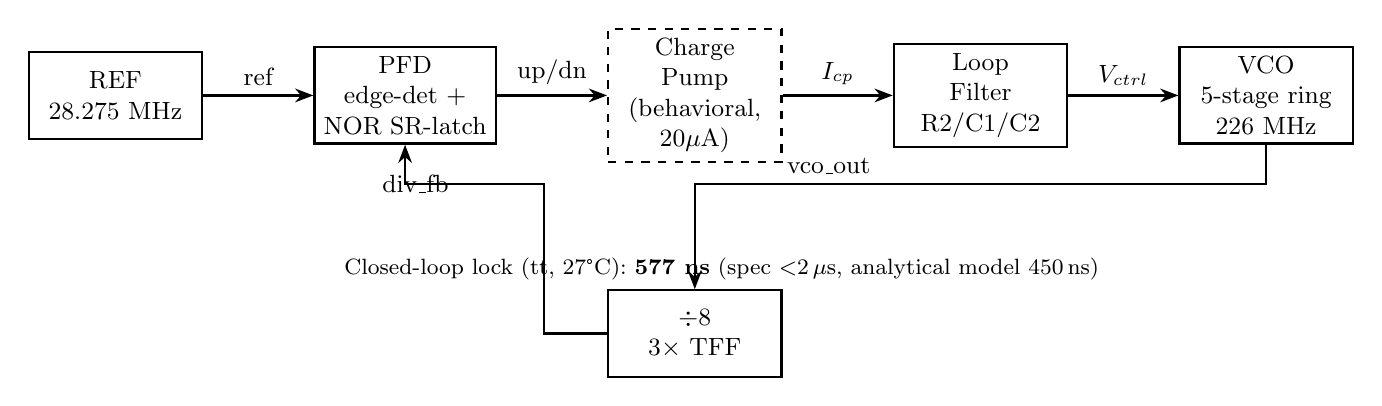
\includegraphics[width=\linewidth]{pll_block_diagram.png}\caption{PLL block diagram. PFD, divider and VCO are transistor-level; the charge pump is behavioural.}\label{fig:blk}\end{figure}

\paragraph{PFD.} Edge detectors feeding a cross-coupled NOR SR latch (instead of resettable D flip-flops, to avoid fighting the latch feedback with an asynchronous reset). Functionally verified by sweeping the phase relationship.

\paragraph{Charge pump (behavioural).} $I_{cp}=20\,\mu$A, an ideal current source gated by UP/DN: no switch resistance, no mismatch, no charge injection. A 5$\times$ boost of the pump current is applied until the first divider edge, so that a true 0\,V start can recover (Fig.~\ref{fig:acq}).
\begin{figure}[!htbp]\centering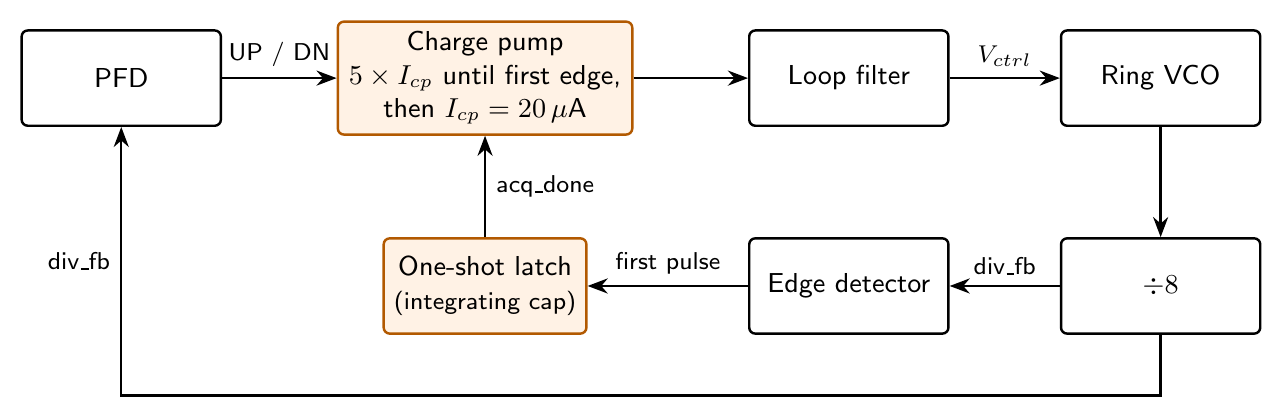
\includegraphics[width=0.85\linewidth]{acq_boost.png}\caption{Acquisition aid: pump current boosted $5\times$ until the first divider edge.}\label{fig:acq}\end{figure}

\paragraph{Loop filter.} $R_2=3.6$\,k$\Omega$ in series with $C_1=68$\,pF, $C_2=6.8$\,pF in parallel. The original $R_2=1.7$\,k$\Omega$ is superseded (Section~6.3).

\paragraph{VCO.} A 5-stage current-starved ring (Fig.~\ref{fig:vco}). $\vc$ drives the NMOS current-source gates directly and, through a V-to-I device and a PMOS mirror, the PMOS current sources, so it sets the delay per stage. Default sizing: switching devices W/L = 1.0/0.5 (N) and 2.0/0.5 (P), current sources 2.0/0.5\,$\mu$m (all sky130 \texttt{nfet\_01v8}/\texttt{pfet\_01v8}); supply current about 58\,$\mu$A at the 0.9\,V bias point. The tuning curve is S-shaped: 18\,MHz at 0.65\,V to 358\,MHz at 1.40\,V (tt), 226.2\,MHz at 0.9\,V, with a local $\kvco\approx890$\,MHz/V at 0.9\,V (tt). There is no hard oscillation floor: 0.63, 2.1, 6.5 and 18\,MHz at 0.50, 0.55, 0.60 and 0.65\,V.
\begin{figure}[!htbp]\centering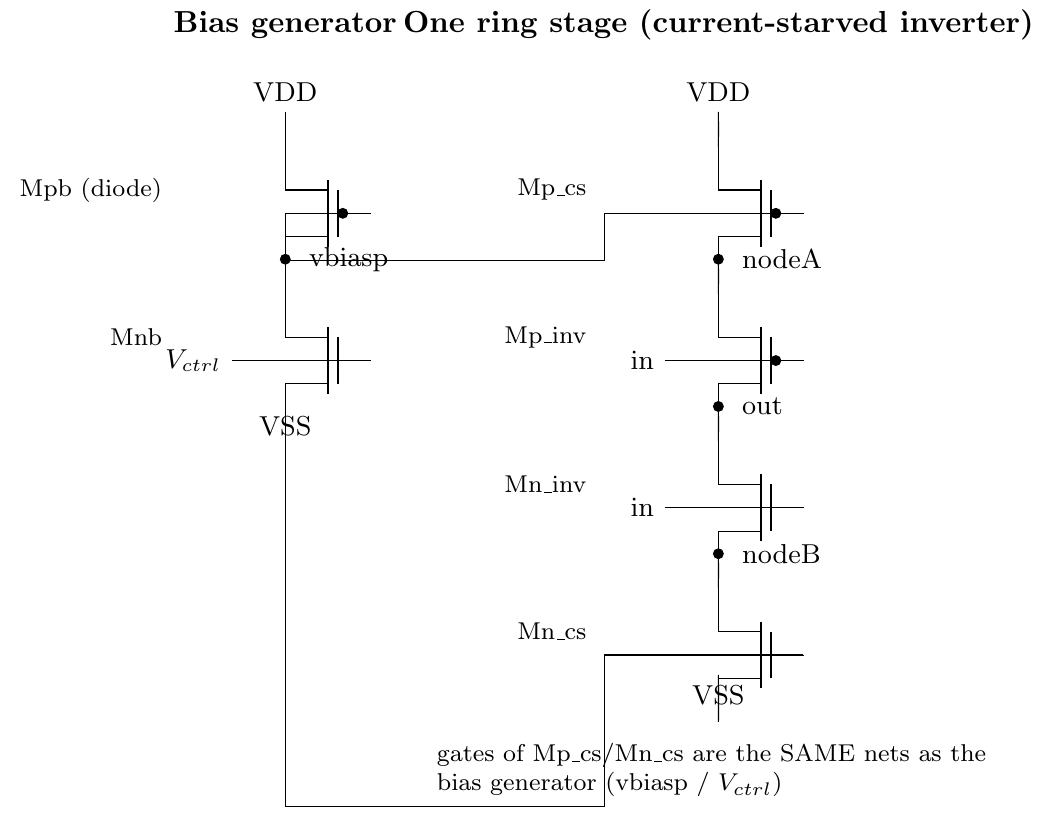
\includegraphics[width=0.46\linewidth]{vco_schematic.png}\hfill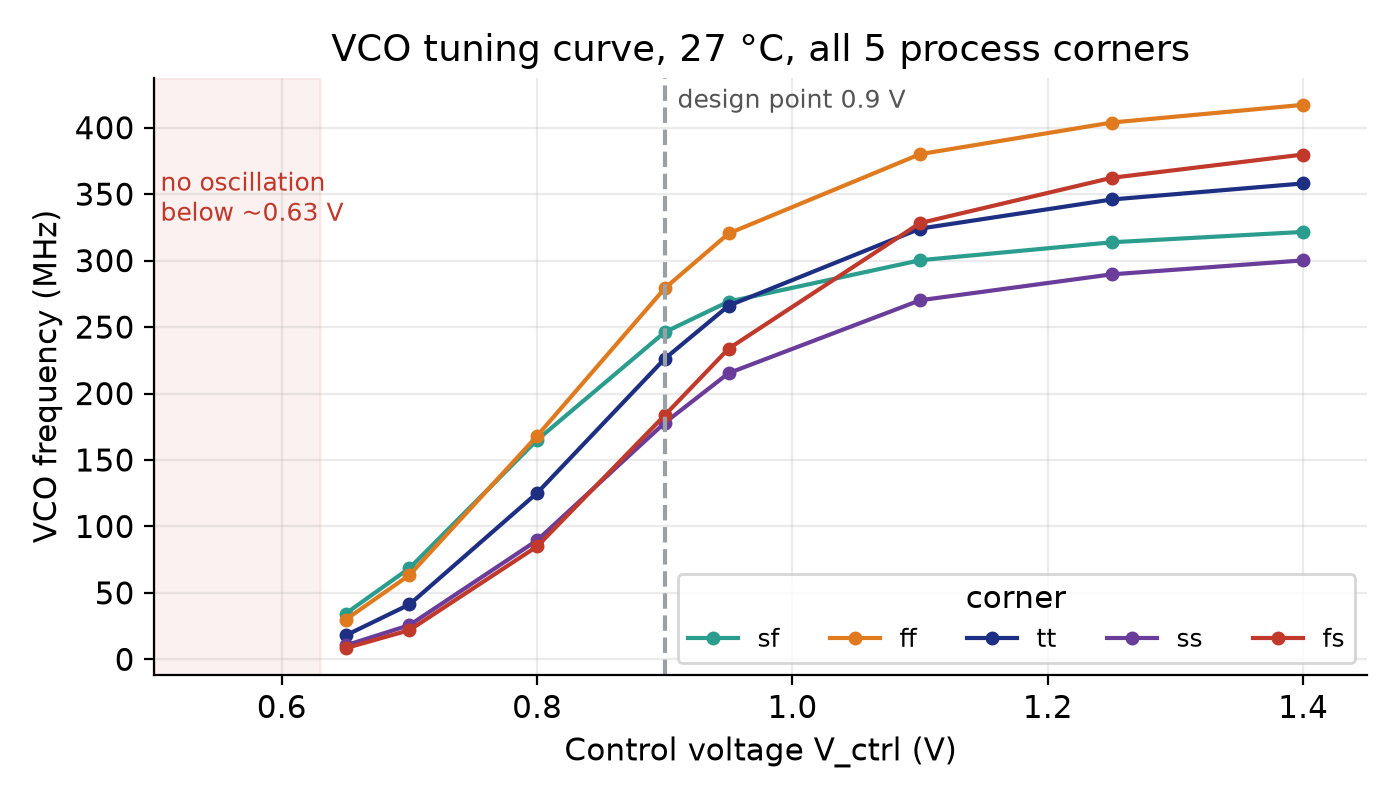
\includegraphics[width=0.52\linewidth]{tuning.png}\caption{Left: current-starved ring VCO. Right: tuning curve at tt, 27\degC.}\label{fig:vco}\end{figure}

\paragraph{Divider.} $\div8$ from three cascaded toggle flip-flops; measured ratio 8.004 in the block test.

\paragraph{Compensation network (behavioural).} In the simulations the correction is an ideal voltage source in series with $\vc$:
\begin{equation}\vc^{\,\mathrm{eff}}=\vc+k_1(T-27)+k_2(T-27)^2.\end{equation}
$k_2=0$ gives a first-order (PTAT/CTAT-equivalent) network. A transistor-level realisation (PTAT/CTAT plus translinear squarer) is proposed in Section~8 (Fig.~\ref{fig:comp}).
\begin{figure}[!htbp]\centering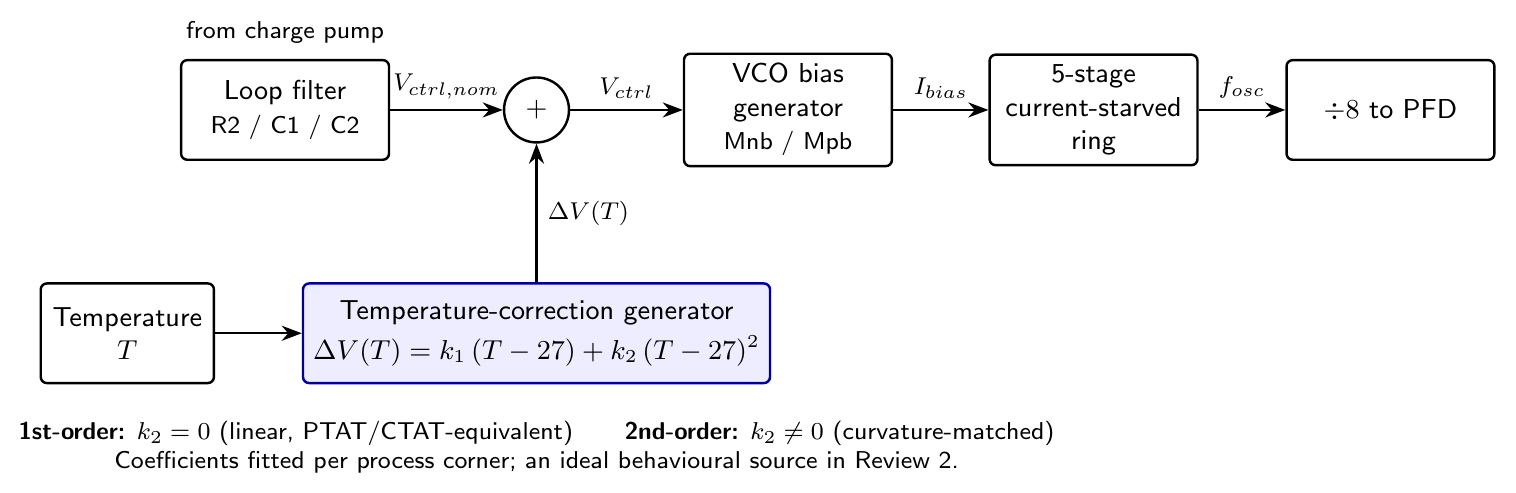
\includegraphics[width=0.9\linewidth]{compensation_arch.png}\caption{Compensation architecture (target realisation; the present simulations use the ideal source of Eq.~1).}\label{fig:comp}\end{figure}

%================== 4 ==================
\section{Methodology}
\subsection{Simulation flow}
Every result is produced by headless ngspice batch runs driven by Python scripts, from netlists under \texttt{blocks/}. Raw outputs and per-run JSON are kept under \texttt{results/}; every headline number is regenerated into \texttt{results/final\_numbers.md} by a script, and the tables in this report are generated from that file. Appendix~A lists the commands.

\subsection{Corner methodology}
sky130 ships the corners ss, tt, ff and two skew corners sf, fs. During the final preparation we found that the VCO results did not look like textbook corners and audited them. We measured the devices directly (Table~\ref{tab:dev}) and found: (a) in this PDK \texttt{sf} is fast-NMOS/slow-PMOS and \texttt{fs} is slow-NMOS/fast-PMOS (measured; our earlier labels were reversed; the PDK documentation does not state it unambiguously); (b) the skew corners shift each device further than ss/ff do: extracted NMOS $V_{th}$ vs tt is $+25$ (ss), $-25$ (ff), $-36$ (sf), $+36$\,mV (fs), PMOS $|V_{th}|$ $+15$, $-23$, $+32$, $-43$\,mV. At the VCO bias (overdrive $\approx0.2$\,V) this becomes $\approx9\,\%$ in drive current, so the PDK skews lie outside the ss--ff envelope at 0.9\,V but inside it at 1.8\,V (NMOS $I_d$ within 1\,\%).

\begin{table}[!htbp]\centering\small
\begin{tabular}{lrrrrrr}\toprule
Corner & N $I_d$ 0.9 V ($\mu$A) & P $I_d$ 0.9 V ($\mu$A) & N $I_d$ 1.8 V ($\mu$A) & P $I_d$ 1.8 V ($\mu$A) & N $V_{th}$ (V) & P $|V_{th}|$ (V) \\\midrule
ss & 27.9 & 0.112 & 401.2 & 69.9 & 0.6945 & 1.3376 \\
sf & 51.3 & 0.082 & 480.0 & 68.5 & 0.6333 & 1.3548 \\
tt & 36.9 & 0.211 & 438.2 & 86.5 & 0.6693 & 1.3229 \\
fs & 25.3 & 0.518 & 397.2 & 104.4 & 0.7054 & 1.2800 \\
ff & 47.7 & 0.403 & 475.4 & 103.2 & 0.6441 & 1.3000 \\
\bottomrule\end{tabular}
\caption{Single-device audit at 27\degC\ (W/L = 2/0.5\,$\mu$m, ngspice~47). Skew corners fall outside the ss--ff band for the NMOS at 0.9\,V (25.3 and 51.3 vs 27.9 and 47.7\,$\mu$A). PMOS at 0.9\,V is sub-threshold.}\label{tab:dev}
\end{table}

We therefore report on \textbf{11 corners}: a textbook $3\times3$ set (NMOS slow/typ/fast $\times$ PMOS slow/typ/fast), named \texttt{nXpY} (\texttt{nsps}=ss, \texttt{ntpt}=tt, \texttt{nfpf}=ff exactly as in the PDK), built by swapping the NMOS and PMOS model files independently (\texttt{scripts/make\_factorial\_lib.py}; the diagonal reproduces the PDK ss/tt/ff to the digit: 177.993/226.206/279.178\,MHz), plus the PDK's own skews as wider ``foundry'' extremes. We always label by device behaviour, never by the letters alone.

\subsection{Compensation fit}
The first analytic coefficients (Review~2) were derived from a wrong $\kvco$ and a first-order guess; they are superseded (Section~6.3). The method now used (\texttt{scripts/comp\_factorial.py}), per corner:
\begin{enumerate}[nosep]
\item measure $f(T,V)$ at $V\in\{0.85,0.90,0.95\}$\,V and $T\in\{-40,-20,0,27,50,85\}$\degC\ (no correction);
\item solve for the exact shift $\Delta V^*(T)$ that restores $f(27\,^\circ\mathrm C)$ (quadratic interpolation in $V$);
\item least-squares fit $\Delta V^*=k_1\Delta T$ (first order) and $k_1\Delta T+k_2\Delta T^2$ (second order), $\Delta T=T-27$;
\item \textbf{verify by simulating} the compensated VCO at the six fit temperatures and at four held-out temperatures ($-30$, 10, 40, 70\degC$)$.
\end{enumerate}
Reported metrics: span $=(f_{max}-f_{min})/f_{27}$ and maximum deviation from $f_{27}$ (the quantity that the $\pm0.3\,\%$ specification refers to), both at $\vc=0.9$\,V. The compensation ratio is $C=$ baseline span / second-order span.

\subsection{Monte Carlo and paired statistics}
Device mismatch is enabled through the PDK's mismatch switch with a fixed random seed set first in each run. Each seed is one simulated chip, run through all three arms (uncompensated, first order, second order) at $-40$ and $85$\degC\ with the tt coefficients; the drift is $|f(85)-f(-40)|$. Arms are \emph{paired by seed}; we use a paired $t$ test with a 95\,\% CI and a Wilcoxon signed-rank test, and the metric is $|{\rm drift}|$ because over- and under-correction are equally bad (our first analysis tested the signed drift and was wrong; Section~6.3). $n=72$ chips. Statistics are hand-written (\texttt{scripts/stats.py}) and self-checked.

\subsection{Closed-loop campaign}
\texttt{scripts/closed\_loop\_campaign.py} runs the full transistor-level loop (behavioural charge pump) at all 11 corners from two start states: a coarse start ($\vc=0.85$\,V) and a true cold start ($\vc=0$\,V, boosted pump); plus cold starts at $-40$ and 85\degC\ for ss, tt, ff. Each run is 5\,$\mu$s. \emph{Lock time} is the time after which $\vc$ stays within $\pm2\,\%$ of its final value (specification $<2\,\mu$s). In total 28 simulations.

%================== 5 ==================
\section{Results}
\subsection{Corner audit and VCO characterisation}
\begin{figure}[!htbp]\centering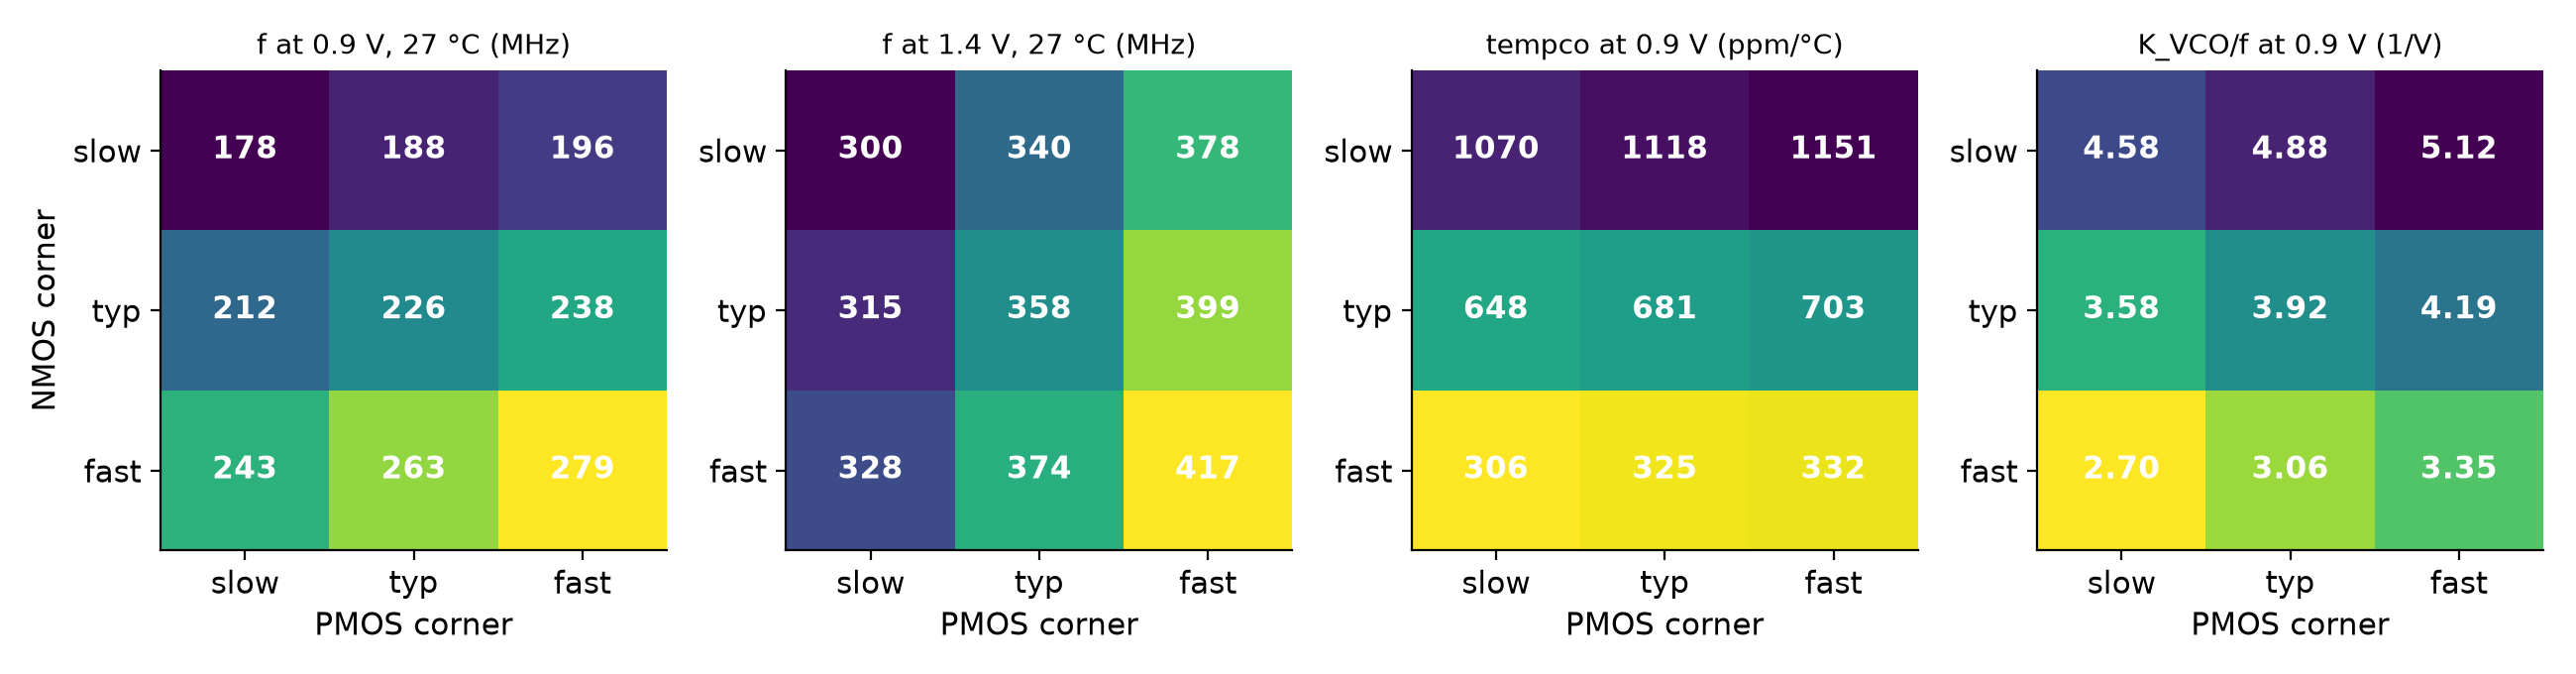
\includegraphics[width=\linewidth]{audit_factorial_maps.png}\caption{Textbook $3\times3$ NMOS$\times$PMOS set. From left: $f$ at 0.9\,V, $f$ at 1.4\,V (27\degC), tempco at 0.9\,V (ppm/\degC), $\kvco/f$ (1/V).}\label{fig:maps}\end{figure}
At 0.9\,V and 27\degC\ the frequency is 178.0/188.0/195.9 (N slow), 211.8/226.2/238.1 (N typ), 242.8/262.7/279.2\,MHz (N fast) for P slow/typ/fast. Tempco is 1070/1118/1151, 648/681/703 and 306/325/332\,ppm/\degC; the textbook range is 306--1151 (3.8$\times$) and the PDK five-corner range is 112 (sf)--1399 (fs) ppm/\degC\ (12.5$\times$), with ss 1070, tt 681 and ff 332. All 8 monotonicity checks pass (frequency rises with NMOS and with PMOS strength at 0.9 and 1.4\,V; tempco falls with NMOS strength). The only failed expectation is that the PDK skews' tempco lies inside $[$ff, ss$]$; it does not, even in a clean textbook set tempco is not bounded by ff and ss. Physics checks pass: $V_{th}$ tempco $-0.78$\,mV/\degC\ (N) and $-1.1$\,mV/\degC\ (P); NMOS $I_d$ at 1.8\,V falls with temperature ($-30\,\%$) while at 0.9\,V it rises ($+14\,\%$), i.e.\ the bias sits below the zero-tempco point; at $\vc=1.4$\,V the tempco is $-816$\,ppm/\degC\ (sign flip). At 0.9\,V the NMOS limits the ring (36\,\% spread slow-to-fast N vs 10\,\% across P); at 1.4\,V the PMOS does (26\,\% vs 9\,\%). Uncompensated at tt the span is 8.51\,\%. Local $\kvco$ at 0.9\,V (MHz/V): sf 580, ff 940, tt 890, ss 820, fs 1020 (the earlier 669 was wrong).
\begin{figure}[!htbp]\centering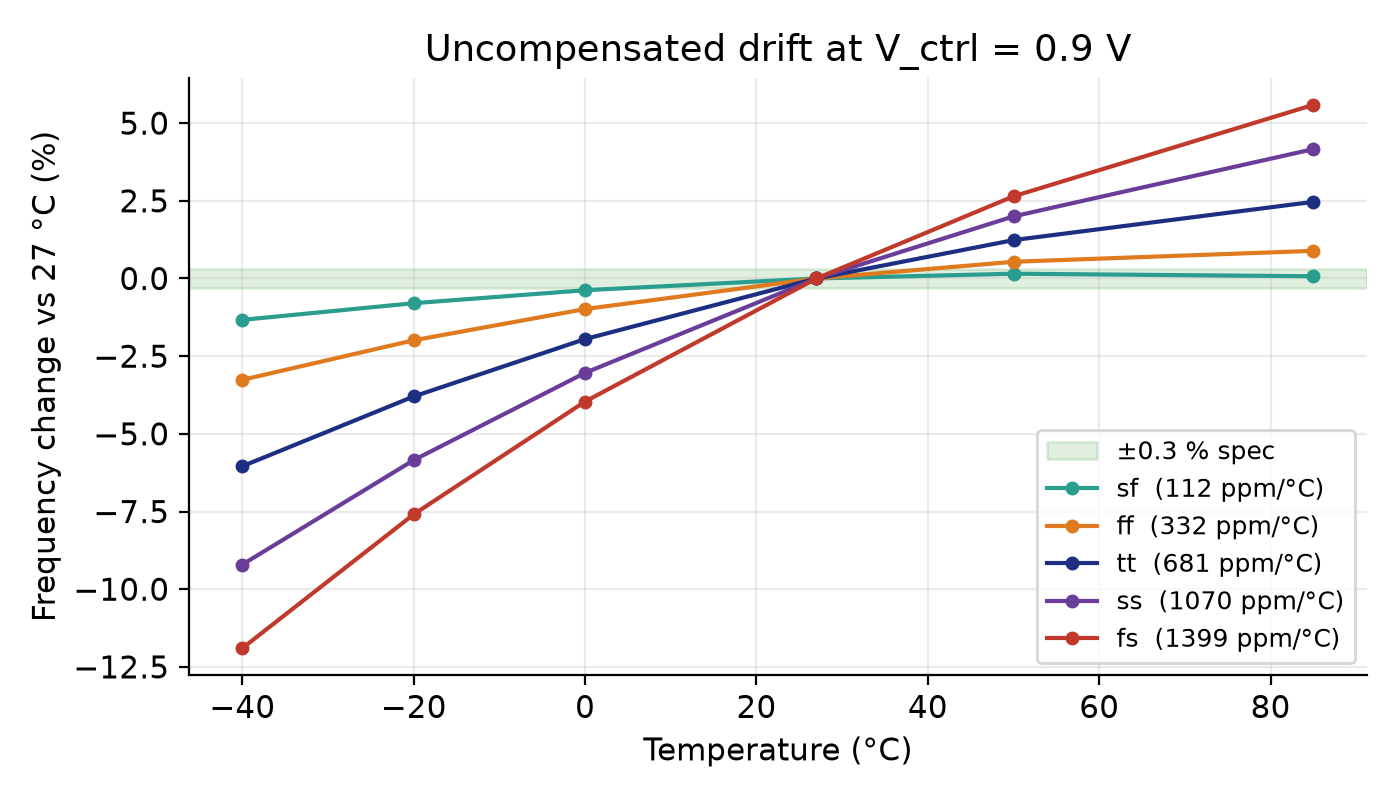
\includegraphics[width=0.49\linewidth]{drift_uncomp.png}\hfill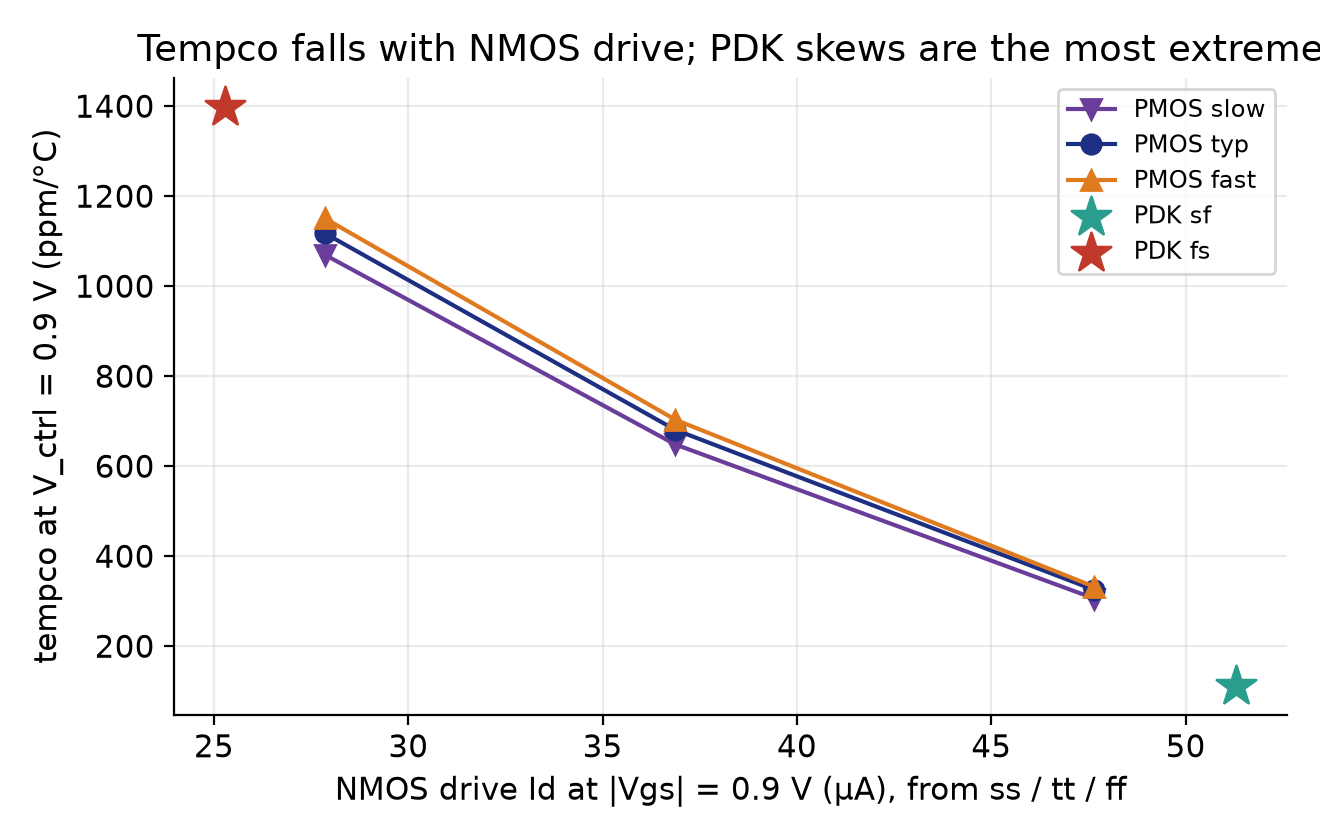
\includegraphics[width=0.49\linewidth]{audit_tempco_vs_nmos.png}\caption{Left: uncompensated VCO drift vs temperature (tt). Right: tempco ranks with NMOS drive.}\label{fig:drift}\end{figure}

\subsection{Compensation on 11 corners}
\begin{table}[!htbp]\centering\small\setlength{\tabcolsep}{4pt}
\begin{tabular}{lrrrrrrl}\toprule
Corner & $f_0$ (MHz) & Base span (\%) & 2nd span (\%) & Max dev (\%) & Held-out (\%) & $C$ & $\pm0.3\,\%$ \\\midrule
nsps (ss) & 178.0 & 13.37 & 0.35 & 0.277 & 0.175 & 38.4 & yes \\
nspt & 188.0 & 13.97 & 0.38 & 0.301 & 0.201 & 37.2 & \textbf{\textcolor{warn}{NO}} \\
nspf & 195.9 & 14.38 & 0.42 & 0.325 & 0.223 & 34.3 & \textbf{\textcolor{warn}{NO}} \\
ntps & 211.8 & 8.10 & 0.24 & 0.195 & 0.109 & 33.6 & yes \\
ntpt (tt) & 226.2 & 8.51 & 0.20 & 0.162 & 0.091 & 43.2 & yes \\
ntpf & 238.1 & 8.79 & 0.20 & 0.168 & 0.097 & 43.7 & yes \\
nfps & 242.8 & 3.82 & 0.12 & 0.079 & 0.034 & 31.0 & yes \\
nfpt & 262.7 & 4.06 & 0.12 & 0.102 & 0.041 & 33.3 & yes \\
nfpf (ff) & 279.2 & 4.15 & 0.11 & 0.093 & 0.035 & 37.0 & yes \\
PDK sf (N fast, P slow) & 246.2 & 1.49 & 0.09 & 0.051 & 0.036 & 15.9 & yes \\
PDK fs (N slow, P fast) & 183.7 & 17.49 & 0.49 & 0.360 & 0.251 & 35.8 & \textbf{\textcolor{warn}{NO}} \\
\bottomrule\end{tabular}
\caption{Compensation, nominal (no mismatch), ideal behavioural source, $\vc=0.9$\,V. ``Max dev'' is the maximum deviation from $f_{27}$ of the second-order-compensated VCO at the 6 fit temperatures; ``Held-out'' the same at $-30$, 10, 40, 70\degC.}\label{tab:comp}
\end{table}
\begin{figure}[!htbp]\centering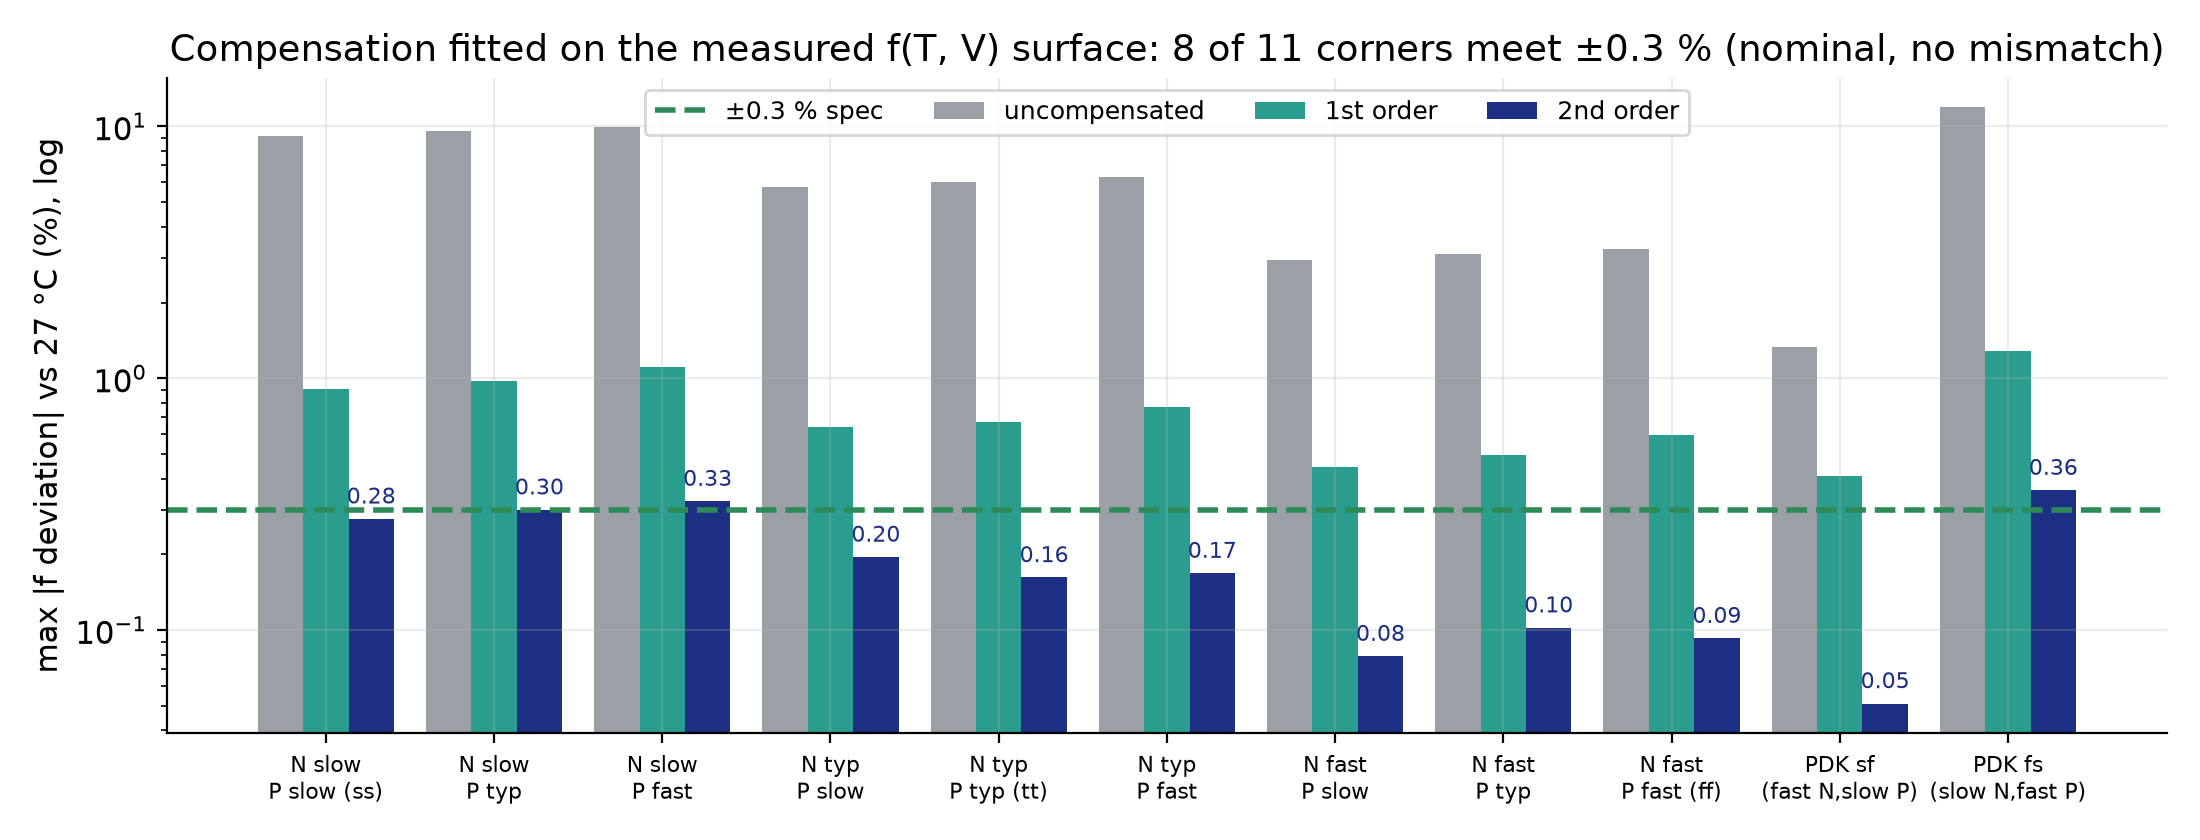
\includegraphics[width=\linewidth]{final_comp_corners.png}\caption{Maximum deviation from $f_{27}$ (log scale) for the uncompensated, first-order and second-order cases at 11 corners.}\label{fig:compc}\end{figure}
At tt the span falls from 8.51\,\% to 0.67\,\% (first order) and 0.20\,\% (second order), maximum deviation 0.16\,\% (specification $\pm0.3\,\%$ met), held-out 0.09\,\%, with $k_1=-1.543\times10^{-4}$\,V/\degC\ and $k_2=4.18\times10^{-7}$\,V/\degC$^2$. \textbf{8 of 11 corners meet $\pm0.3\,\%$} (7 of the 9 textbook corners). The misses are \texttt{nspt} 0.301\,\% (borderline), \texttt{nspf} 0.325\,\% and PDK fs 0.360\,\%; all are slow-NMOS corners, the hardest. $C$ lies between 31 and 44 for ten corners and is 15.9 for PDK sf (small baseline drift). Held-out maxima are 0.03--0.25\,\%, so the two fitted coefficients do not over-fit the five non-reference fit temperatures. Per-corner coefficients are in Appendix~B.

\begin{miss}{Caveats on this result}
The correction is an ideal source (no transistor-level network, no noise, no supply dependence); it is nominal (no mismatch); two coefficients are fitted to five temperature points; and the fit is made at $\vc=0.9$\,V while each corner locks at its own $\vc$ (Section~5.4).
\end{miss}

\subsection{Monte Carlo, $n=72$, and the mismatch floor}
\begin{figure}[!htbp]\centering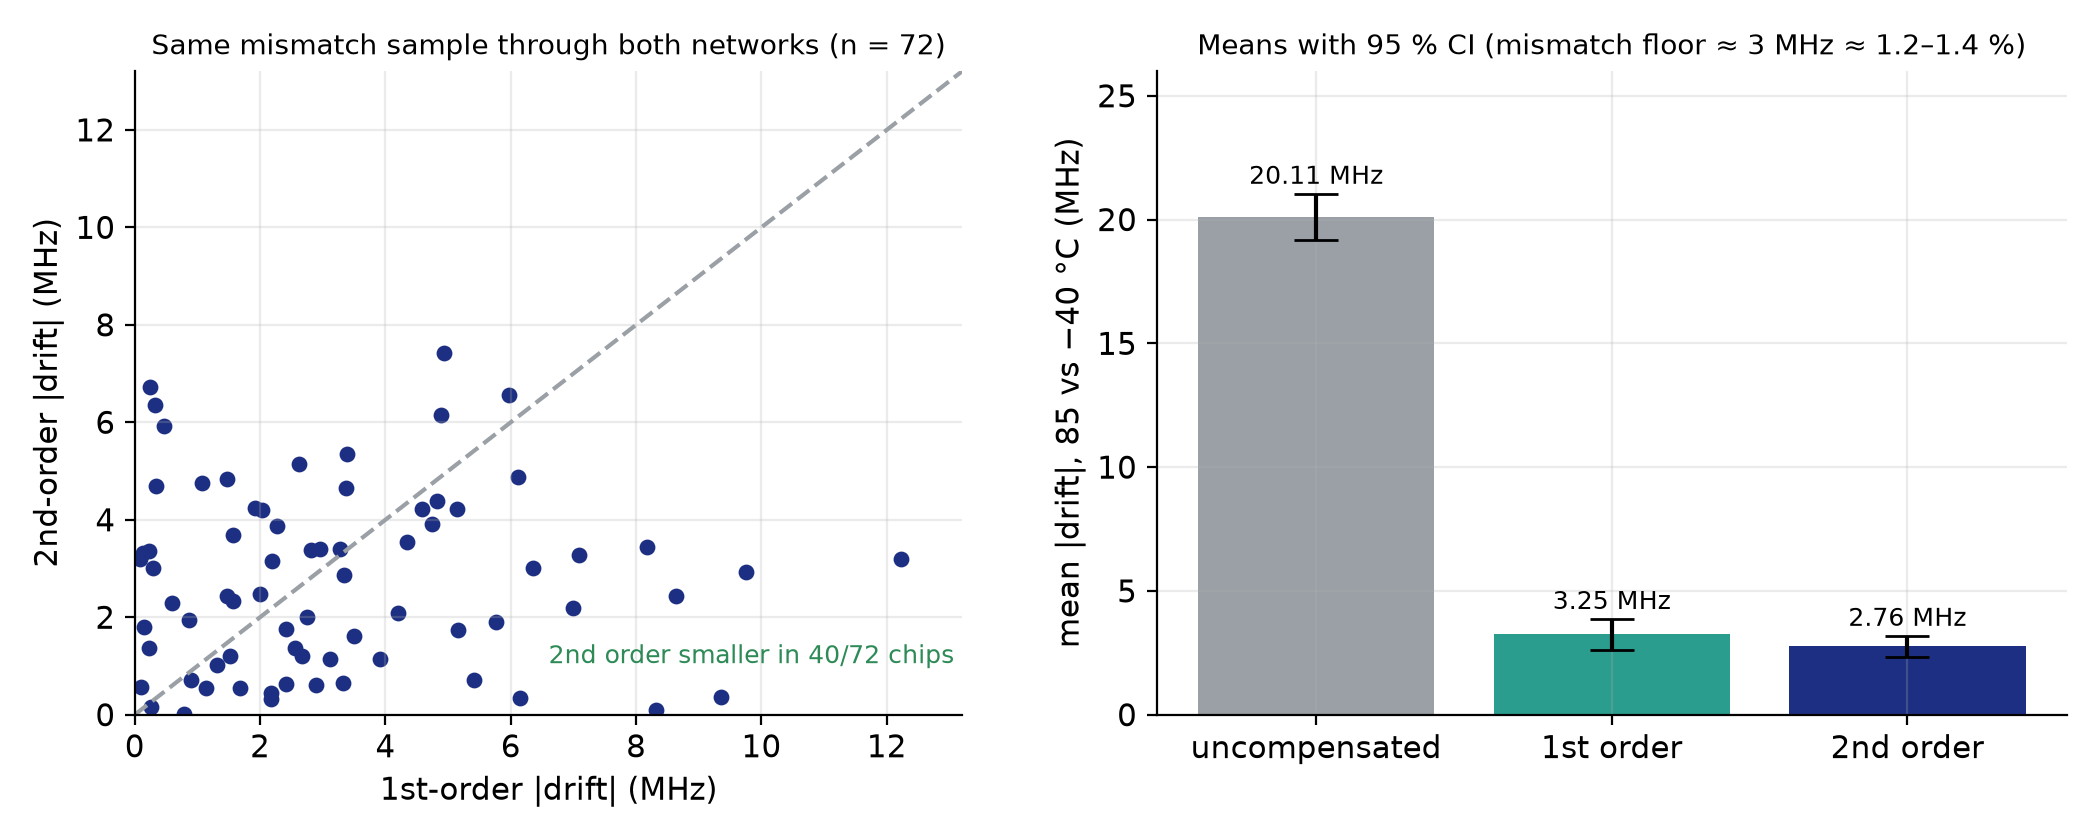
\includegraphics[width=\linewidth]{final_mc.png}\caption{Monte Carlo at tt with mismatch ($n=72$ chips, paired by seed). Left: second- vs first-order $|$drift$|$ per chip. Right: means with 95\,\% CI.}\label{fig:mc}\end{figure}
\begin{table}[!htbp]\centering\small
\begin{tabular}{lrrl}\toprule
Arm & mean $|$drift$|$ (MHz) & 95\,\% CI (MHz) & as \% of 226.2\,MHz\\\midrule
Uncompensated & 20.11 & [19.18, 21.04] & --\\
First order & 3.25 & [2.63, 3.87] & 1.4\\
Second order & 2.76 & [2.33, 3.19] & 1.2\\\bottomrule
\end{tabular}\quad
\begin{tabular}{lrl}\toprule
Paired comparison & reduction (MHz), CI & wins\\\midrule
Base $\to$ 1st & 16.86 [15.57, 18.16] & 71/72\\
Base $\to$ 2nd & 17.35 [16.37, 18.34] & 72/72\\
1st $\to$ 2nd & 0.49 [$-0.26$, 1.24], n.s. & 40/72\\\bottomrule
\end{tabular}
\caption{Monte Carlo statistics. Both $t$ and Wilcoxon tests agree: both compensations significantly reduce drift; 1st $\to$ 2nd is not significant.}\label{tab:mc}
\end{table}
Either compensation removes 84--86\,\% of the drift under mismatch, in nearly every chip. But the residual of about 3\,MHz (1.2--1.4\,\% of 226\,MHz) is several times the nominal residual (0.2--0.7\,\%): it is a \textbf{mismatch floor}. Chip-to-chip mismatch makes every chip's own drift differ (signed drift std 4.1\,MHz first order, 3.3\,MHz second order), and one global correction cannot remove a per-chip error. With correctly fitted coefficients the second-order term gives \emph{no statistically detectable benefit under mismatch}. Reaching $\pm0.3\,\%$ across chips would require per-chip trim (Section~8.4). Monte Carlo was run at the tt corner only.

\subsection{Closed loop}
\paragraph{Retune.} The Review-1 filter design had dropped the $1/(2\pi)$ of the PFD/charge-pump gain, so $\zeta$ was 0.33, not 0.72. Retuning $R_2$ from 1.7 to 3.6\,k$\Omega$ gives $\zeta\approx0.70$ (phase margin $\approx$65--70$^\circ$ by the $100\zeta$ rule, not a Bode plot). At tt: coarse-start lock 577\,$\to$\,503\,ns, cold start 839\,$\to$\,1351\,ns (slower but within specification), ripple 8.6\,$\to$\,0.35\,mV, final frequency error 0.78\,\%\,$\to$\,0.008\,\%. The original loop had not settled within 2\,$\mu$s at ff, sf, fs, ss. Only $R_2=1.7$, 3.0 and 3.6\,k$\Omega$ were simulated at transistor level; 3.6\,k$\Omega$ is not claimed optimal.

\paragraph{Lock at all corners.} In all 28 runs $\fvco=226.17$\,MHz ($-0.01\,\%$, the bias of the crossing detector) $=8f_{ref}$, ripple $\le0.8$\,mV, all settled. Lock times at 27\degC\ are in Table~\ref{tab:lock} and Fig.~\ref{fig:lock}; all are below 2\,$\mu$s.
\begin{table}[!htbp]\centering\small
\begin{tabular}{lrrr}\toprule
Corner & $V_{lock}$ (V) & Coarse start (ns) & Cold start (ns) \\\midrule
nsps (ss) & 0.968 & 967 & 1675 \\
nspt & 0.944 & 645 & 1531 \\
nspf & 0.930 & 573 & 1354 \\
ntps & 0.920 & 678 & 1537 \\
ntpt (tt) & 0.900 & 503 & 1351 \\
ntpf & 0.888 & 177 & 1318 \\
nfps & 0.877 & 387 & 1391 \\
nfpt & 0.860 & 279 & 1316 \\
nfpf (ff) & 0.849 & 241 & 1282 \\
PDK sf (N fast, P slow) & 0.869 & 419 & 1388 \\
PDK fs (N slow, P fast) & 0.942 & 576 & 1355 \\
\bottomrule\end{tabular}\quad\begin{tabular}{lrrr}\toprule
Corner & $-40\,^\circ$C & $27\,^\circ$C & $85\,^\circ$C \\\midrule
ss & 1633 & 1675 & \textbf{\textcolor{warn}{2083}} \\
tt & 1318 & 1351 & 1418 \\
ff & 1248 & 1282 & 1317 \\
\bottomrule\end{tabular}
\caption{Top: lock voltage and lock time at 27\degC\ by corner. Bottom: cold-start lock time (ns) vs temperature. The ss/85\degC\ case \textbf{misses the 2\,$\mu$s specification by 4\,\%} (2083\,ns).}\label{tab:lock}
\end{table}
\begin{figure}[!htbp]\centering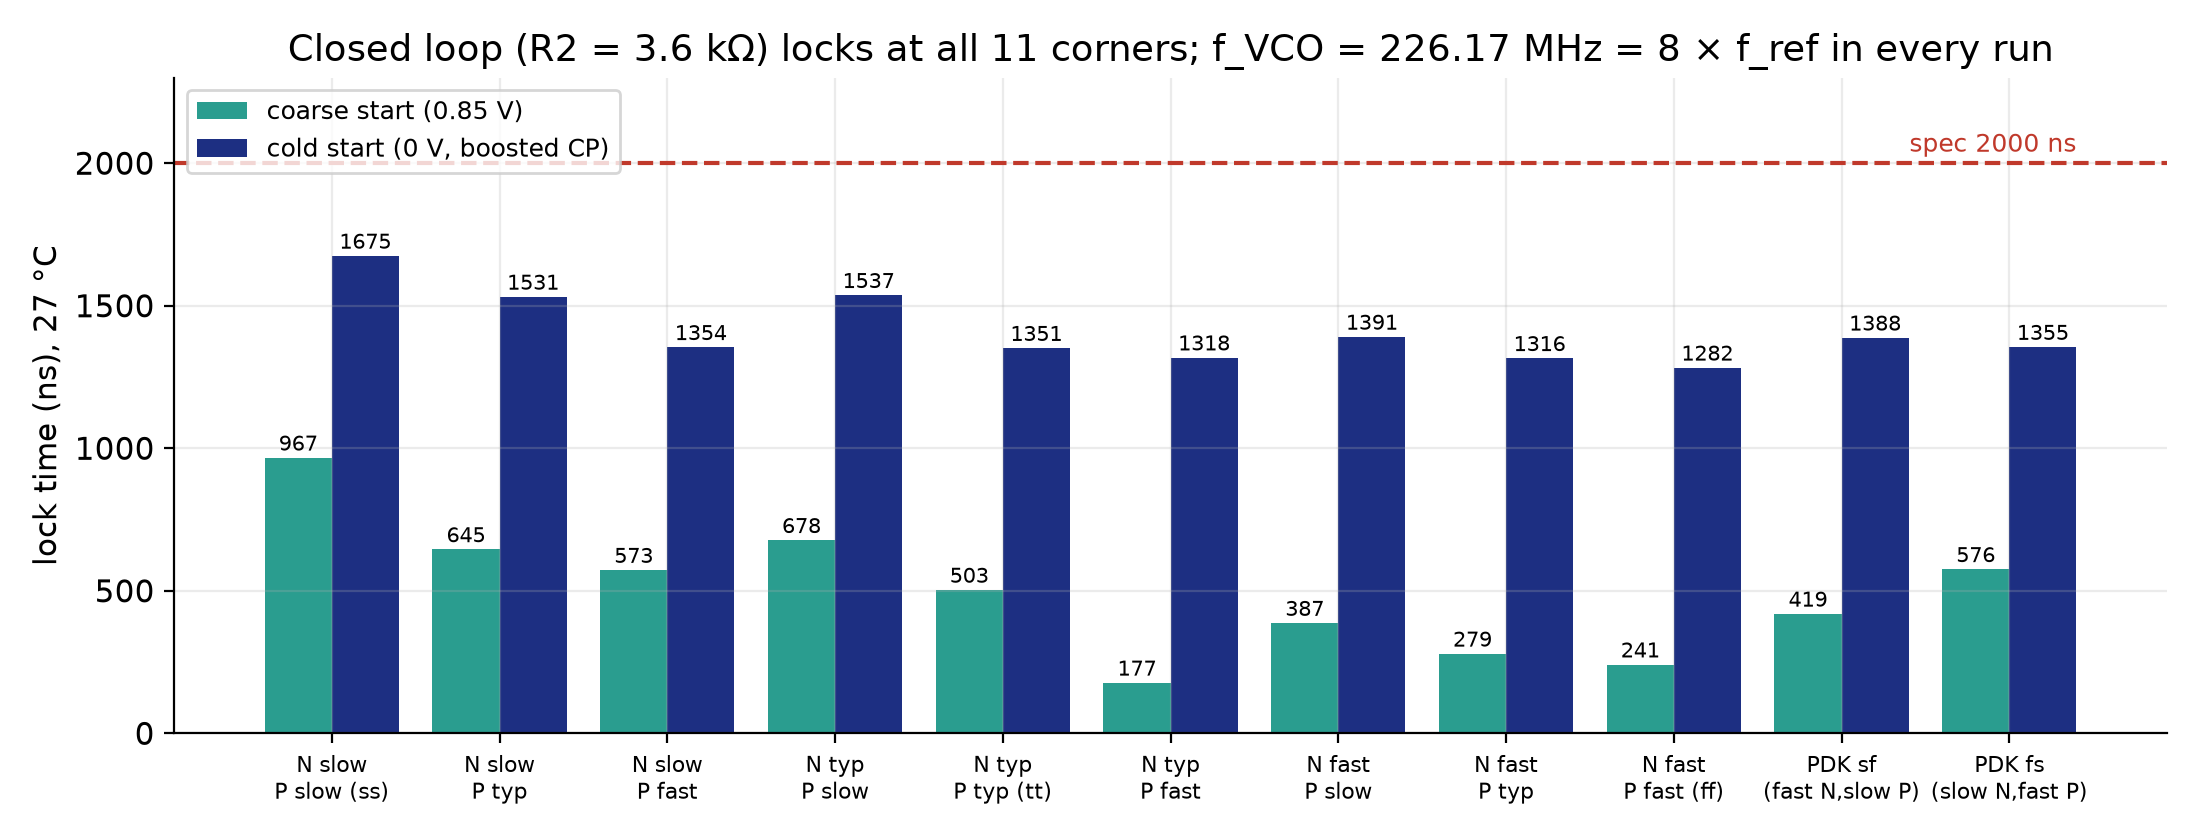
\includegraphics[width=\linewidth]{final_lock_corners.png}\caption{Lock time at 27\degC\ for coarse and 0\,V cold start at the 11 corners.}\label{fig:lock}\end{figure}
\begin{figure}[!htbp]\centering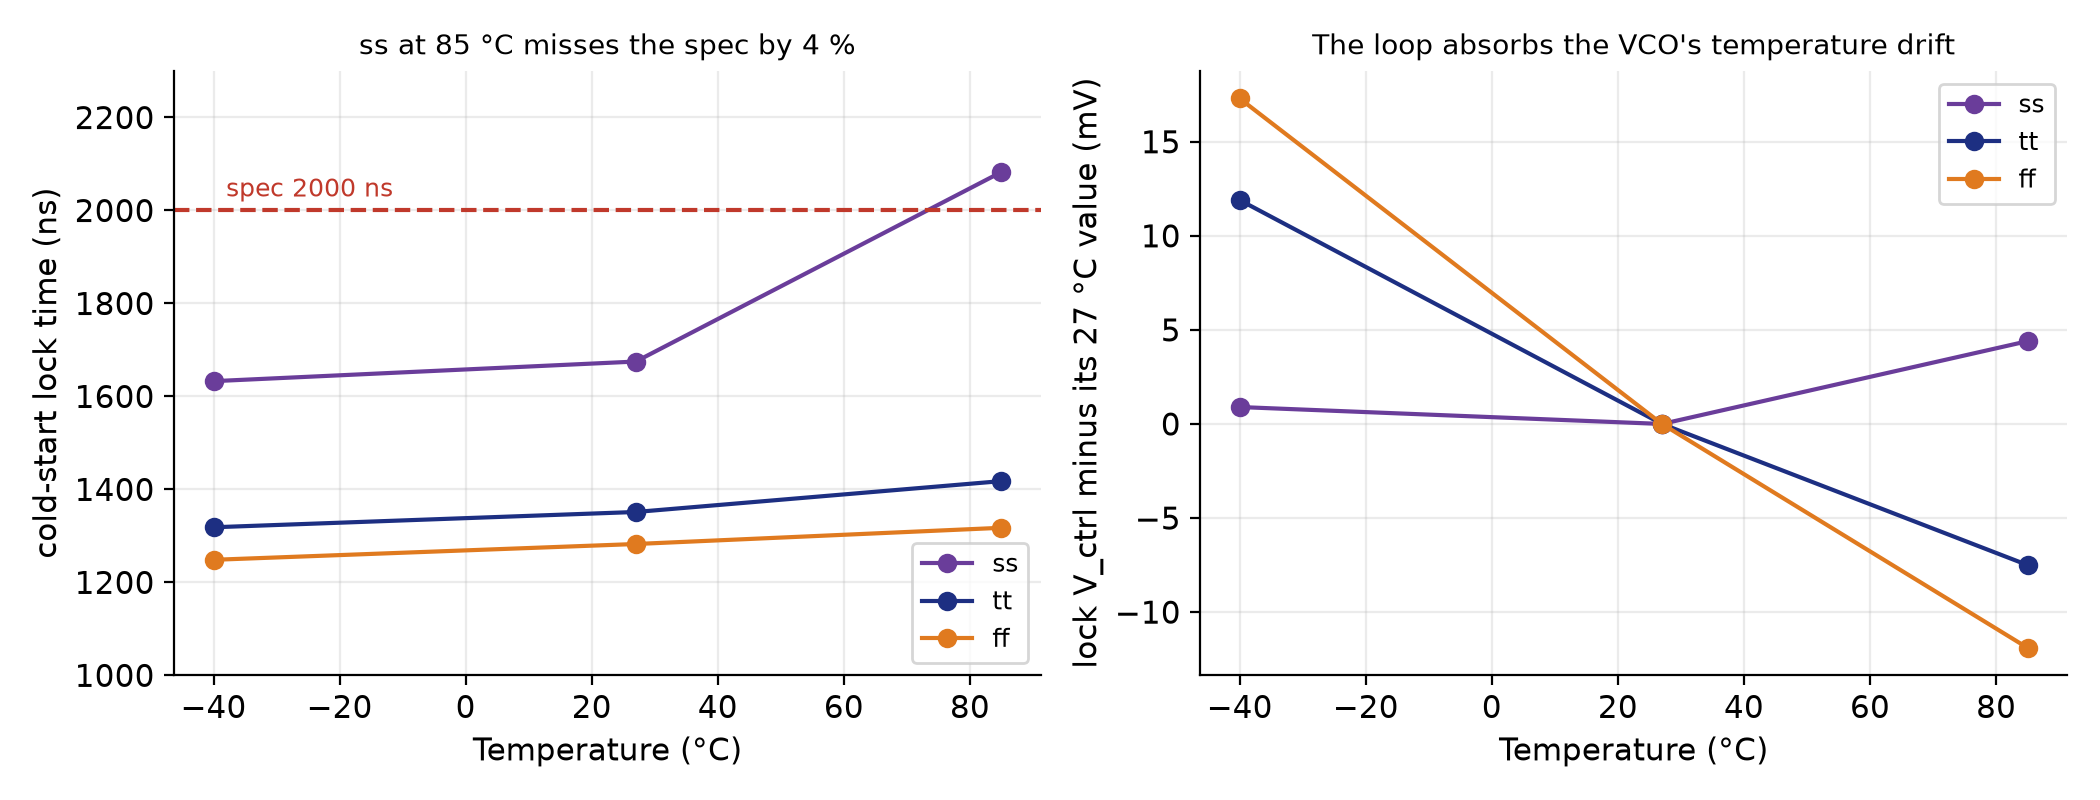
\includegraphics[width=\linewidth]{final_lock_temp.png}\caption{Left: cold-start lock time vs temperature (ss misses at 85\degC). Right: the lock $\vc$ shifts by an amount that absorbs the VCO's drift.}\label{fig:lockT}\end{figure}

\paragraph{Validation checks.} (i)~The closed-loop lock $\vc$ equals the open-loop $\vc$ for 226.2\,MHz within 0.2\,mV at all 11 corners (Fig.~\ref{fig:vlock}). (ii)~At tt the lock voltage moves $+11.9$\,mV at $-40$\degC\ and $-7.5$\,mV at 85\degC, matching the fitted compensation correction at tt ($+12.2$/$-7.5$\,mV): an independent confirmation of the compensation fit \emph{at tt}. At other corners the comparison is not valid because the compensation is fitted at 0.9\,V whereas each corner locks at its own $\vc$ (ss 0.968, nspt 0.944, nspf 0.930, ntps 0.920, tt 0.900, ntpf 0.888, nfps 0.877, nfpt 0.860, ff 0.849, PDK sf 0.869, PDK fs 0.942\,V). This motivates defining the compensation target at each corner's own lock voltage (Section~8.5). (iii)~An earlier averaged behavioural model of the loop reproduced the original 577\,ns lock to within 1\,\% (573\,ns).
\begin{figure}[!htbp]\centering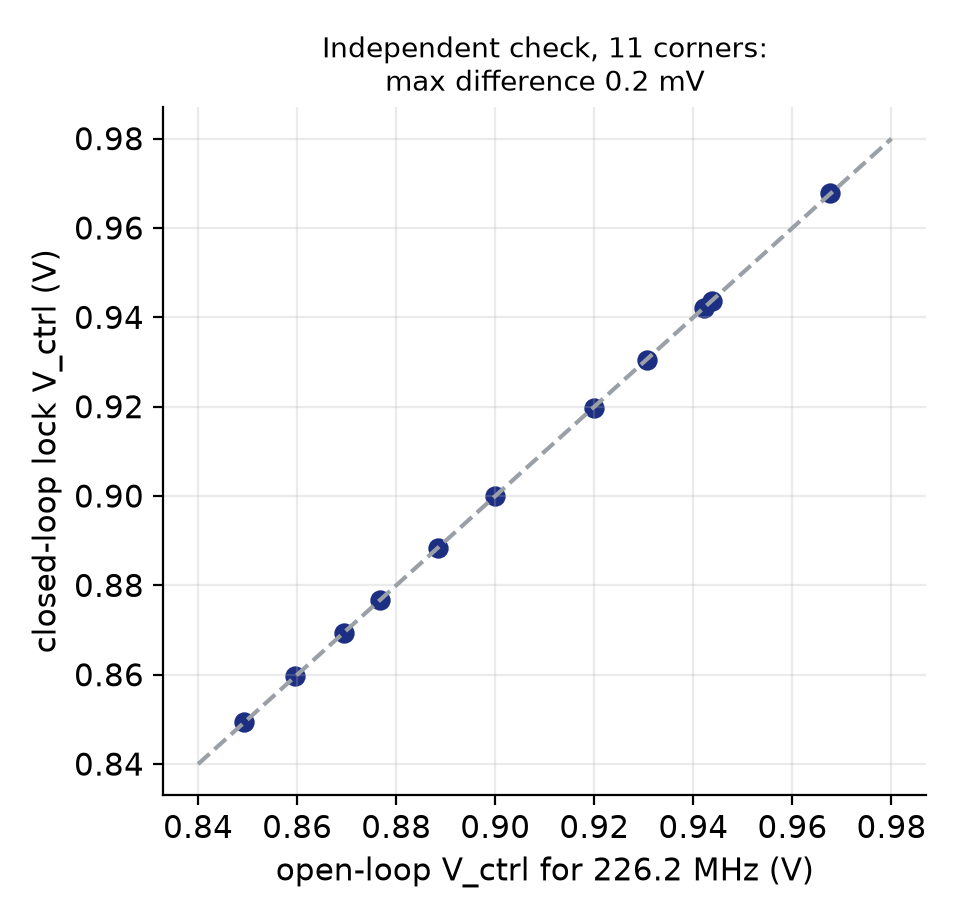
\includegraphics[width=0.42\linewidth]{final_vlock_check.png}\hfill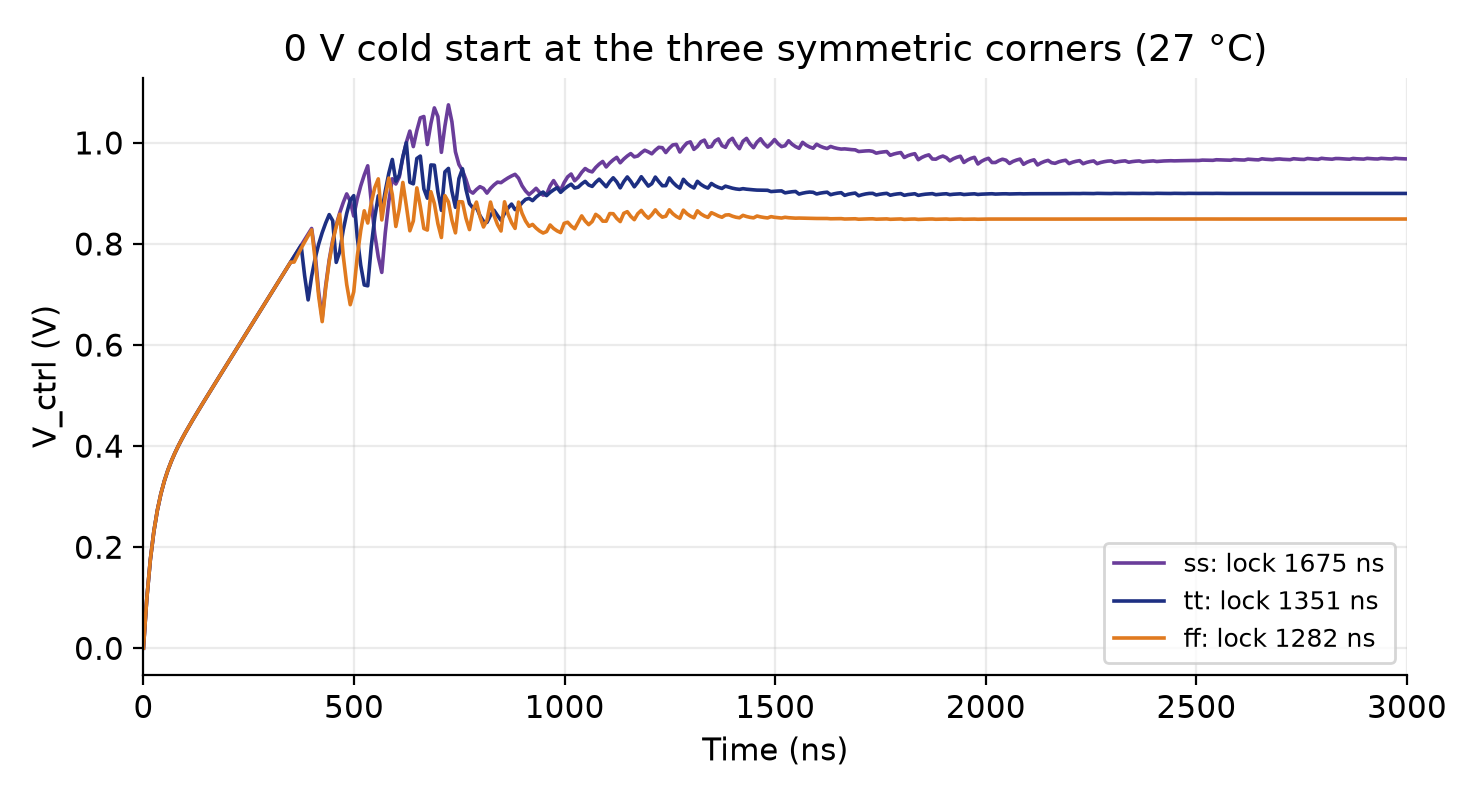
\includegraphics[width=0.56\linewidth]{final_cold_traces.png}\caption{Left: closed-loop vs open-loop lock $\vc$ at 11 corners. Right: 0\,V cold start at ss, tt, ff.}\label{fig:vlock}\end{figure}

%================== 6 ==================
\section{Discussion}
\subsection{What the numbers mean}
The locked output frequency does not drift; what the PLL does is move $\vc$ to absorb the VCO's drift, and compensation reduces how far $\vc$ has to move. Process, not temperature, dominates the lock voltage: across corners $\vc$ at lock spans 0.849--0.968\,V (119\,mV), while temperature moves it by about 20\,mV at tt. All lock voltages stay well above the 0.63\,V practical floor, so lock range was not the limit in any simulated case. The loop closes in every case, and its dynamics move with process because $\kvco$ varies from 580 to 1020\,MHz/V. The weak spot is a slow-NMOS, hot cold start (ss, 85\degC).

\subsection{Comparison with the literature (honest)}
The only cleanly comparable metric is residual frequency variation over temperature. Souliotis et al.\ measured $-1.5\,\%/+0.4\,\%$ (about 1.9\,\% total) over a wider range, $-40$ to 120\degC\ \cite{souliotis22}; Stancu et al.\ report 1.6\,\% in simulation \cite{stancu23}. Our uncompensated tt span of 8.51\,\% is worse than both, as expected. Our compensated nominal span (0.20\,\% at tt) is far below them, but this is a simulation of an \emph{ideal} network, with no mismatch, noise or supply dependence, against \emph{measured silicon} \cite{souliotis22}: it must not be read as beating published silicon. The number that is comparable in spirit is the mismatch-limited 1.2--1.4\,\%, which is in the range of \cite{souliotis22,stancu23}, still from simulation of an ideal network. Lock time ($<2\,\mu$s; 503\,ns coarse, 1351\,ns cold at tt) meets the figure quoted by \cite{geng18}, which is measured silicon at a much higher output frequency. We have no phase-noise number for comparison. The benchmark table is in \texttt{docs/benchmark\_table.md} (it needs updating to the final numbers).

\subsection{Corrections we made, and what they teach}
\begin{enumerate}[nosep]
\item \textbf{sf/fs labels were reversed.} \emph{Lesson:} measure what a model name means; do not assume it.
\item \textbf{Tempco mechanism rewritten:} it follows NMOS overdrive, not N/P current-source balance.
\item \textbf{$\kvco$ 669 $\to$ $\approx890$\,MHz/V.} The 669 came from a fit over the whole S-shaped curve; the local slope at the operating point is what matters.
\item \textbf{No hard 0.63\,V oscillation floor.} It was an artefact of a short simulation window.
\item \textbf{Loop design dropped $1/(2\pi)$:} $\zeta$ was 0.33 not 0.72; retuned to 0.70. Independent re-derivation caught it.
\item \textbf{Compensation coefficients were mis-estimated} through the wrong $\kvco$ and a first-order guess; the new fit meets the specification at tt (0.16\,\%) and 8 of 11 corners. The Review-2 tt values (1.12\,\% span, 0.87\,\% max deviation, specification missed) are superseded.
\item \textbf{Monte Carlo repeated with correct coefficients:} the Review-2 claim ``second order significantly better than first (23/30 seeds)'' compared against a mis-tuned first-order arm and is withdrawn; at $n=72$ it is not significant. (An earlier error, testing signed instead of absolute drift, had also been corrected.)
\item \textbf{PDK skew corners are wider than ss/ff,} not inside the envelope; the textbook $3\times3$ set was added.
\item \textbf{The closed-loop campaign found that ss/85\degC\ cold start misses 2\,$\mu$s by 4\,\%.} \emph{Lesson:} test the worst corner and temperature together, not separately.
\end{enumerate}
Common thread: derived quantities (analytic coefficients, damping, expected corner order) were wrong more often than simulated ones, and each was caught by an independent numerical check. The plan in Section~8 keeps that practice.

\subsection{Threats to validity}
\begin{itemize}[nosep]
\item \emph{Ideal blocks.} Compensation and charge pump are behavioural; transistor-level versions may change every number in Sections~5.2--5.4.
\item \emph{Single simulator, single model set.} ngspice with the legacy per-corner PDK models. The PDK also ships ``continuous'' parameter files with different skew deltas (NMOS $V_{th}$ $\pm15$\,mV for ss/ff vs $\pm27$\,mV for sf/fs); the qualitative story is the same, but the numbers would differ. This is exactly what the planned Spectre arm tests.
\item \emph{Nominal fit, Monte Carlo at one corner.} Mismatch was not run at other corners; the fit is at $\vc=0.9$\,V only.
\item \emph{Few temperature points.} Two coefficients fitted to five points, mitigated by the held-out check.
\item \emph{Lock metric.} The $\pm2\,\%$ band is sensitive at its edge (the 503\,ns tt result is set by a small overshoot just outside the band); damping uses the $100\zeta$ rule, not a Bode plot.
\item \emph{Temperature coverage of closed loop.} Cold start at $\pm$ temperature was simulated at three corners only; not all 11 corners at all temperatures.
\item \emph{Corner definitions.} SkyWater's published documentation of the corner columns is internally inconsistent; we rely on our own measurements.
\end{itemize}

%================== 7 ==================
\section{Research findings summary}
\begin{enumerate}
\item Locked output frequency is $8f_{ref}$ to within $-0.01$\,\% in all 28 simulated cases; temperature acts through $\vc$, $\kvco$ and lock time, not the output frequency.
\item The uncompensated VCO tempco spans 12.5$\times$ across the PDK corners (112--1399\,ppm/\degC) and 3.8$\times$ in a textbook $3\times3$ set (306--1151\,ppm/\degC); tt span is 8.51\,\%.
\item sky130's skew corners are wider than ss/ff (NMOS $V_{th}$ $\pm36$ vs $\pm25$\,mV) and fall outside the ss--ff envelope by 8--9\,\% in drive at the 0.9\,V bias, but within 1\,\% at 1.8\,V.
\item Tempco ranks with NMOS drive at 0.9\,V (NMOS overdrive dominates) and the limiting device flips to the PMOS at 1.4\,V; at $\vc=1.4$\,V the tempco changes sign ($-816$\,ppm/\degC).
\item An ideal second-order correction fitted on measured $f(T,V)$ reduces the nominal tt span from 8.51\,\% to 0.20\,\% (max deviation 0.16\,\%, held-out 0.09\,\%).
\item The $\pm0.3\,\%$ specification is met nominally at 8 of 11 corners and missed at \texttt{nspt} (0.301\,\%), \texttt{nspf} (0.325\,\%) and PDK fs (0.360\,\%).
\item Compensation ratios are 31--44 at ten corners (15.9 at PDK sf).
\item Under mismatch ($n=72$, tt), mean $|$drift$|$ falls from 20.11\,MHz to 3.25\,MHz (first order) and 2.76\,MHz (second order), in 71/72 and 72/72 chips.
\item The residual is a mismatch floor of about 1.2--1.4\,\% (about 3\,MHz), several times the nominal residual (0.2--0.7\,\%), and the second order is not significantly better than the first (0.49\,MHz, CI $[-0.26,1.24]$, 40/72 chips).
\item The retuned loop ($R_2=3.6$\,k$\Omega$, $\zeta\approx0.70$) locks to $8f_{ref}$ at all 11 corners from a coarse start (177--967\,ns) and a 0\,V cold start (1282--1675\,ns) at 27\degC.
\item The worst case, ss at 85\degC\ cold start, takes 2083\,ns and misses the 2\,$\mu$s specification by 4\,\%.
\item Closed-loop lock $\vc$ equals the open-loop value within 0.2\,mV at 11 corners; at tt its temperature shift ($+11.9$/$-7.5$\,mV) equals the fitted correction ($+12.2$/$-7.5$\,mV).
\item Corners lock between 0.849 and 0.968\,V while compensation is fitted at 0.9\,V, so the compensation target should be defined at each corner's own lock voltage.
\end{enumerate}

%================== 8 ==================
\section{Proposal for the remaining work}
All items are proposed; targets are for discussion with the guide. Everything stays in the existing flow, so each item re-uses the scripts of Appendix~A.

\subsection{Transistor-level compensation network (PTAT/CTAT plus squarer)}
\emph{Deliverable:} netlist of a PTAT/CTAT current generator and a translinear squarer driving $\vc^{\,\mathrm{eff}}$, replacing Eq.~1, with $k_1$, $k_2$ set by device ratios and bias. \emph{Acceptance:} nominal tt maximum deviation $\le0.3\,\%$ over $-40$ to 85\degC\ with the network in the loop, held-out points included; agreement with the ideal-source result of Table~\ref{tab:comp} reported; re-run at the 11 corners and the misses of Table~\ref{tab:comp} stated, not hidden. Novelty guard: the patent \cite{ortner17} is cited and our claim stays the composite of Section~2.

\subsection{Transistor-level charge pump}
\emph{Deliverable:} switch-level pump with UP/DN current matching, keeping the $5\times$ acquisition boost. \emph{Acceptance:} lock at tt, ss and ff from 0\,V in $<2\,\mu$s, final frequency error $<0.1\,\%$, ripple reported; the loop campaign of Section~4.5 re-run with the new pump and the ss/85\degC\ case re-checked (it may need a larger boost or a changed $R_2$).

\subsection{Specification restatement (sign-off request)}
Replace $\pm0.15$\,ppm (a reference property in a locked PLL) with: residual VCO free-running drift $\le\pm0.3\,\%$ ($\approx\pm24$\,ppm/\degC) over $-40$ to 85\degC\ and, as loop-level metrics, $\vc$ within $[0.35V_{DD},0.85V_{DD}]\approx[0.63,1.53]$\,V (revised from an original floor of $0.15V_{DD}$ because the ring is below 18\,MHz under 0.65\,V), lock time $<2\,\mu$s, $\kvco$ variation tracked. We ask the guide to confirm both revisions.

\subsection{Per-chip trim to beat the mismatch floor}
\emph{Deliverable:} a trim scheme (for example a few-bit trim of $k_1$ and the squarer gain, set from a one-point or two-point temperature measurement) evaluated by Monte Carlo. \emph{Acceptance:} on $\ge72$ paired chips, $|f(85)-f(-40)|\le1.36$\,MHz (0.6\,\%, i.e.\ $\pm0.3\,\%$ endpoints) for the large majority of chips (target 90\,\%), against 2.76\,MHz untrimmed; the trim range, resolution and the test cost it implies are stated.

\subsection{Compensation at each corner's lock voltage}
\emph{Deliverable:} refit $k_1,k_2$ at each corner's own lock $\vc$ (0.849--0.968\,V, Section~5.4) with the same verification method. \emph{Acceptance:} nominal maximum deviation reported at all 11 corners at their own $\vc$; the three current misses re-assessed; the closed-loop lock-voltage shift of Fig.~\ref{fig:lockT} compared against the fitted correction at \emph{every} corner, not only tt.

\subsection{Layout, DRC, LVS and post-layout}
\emph{Deliverable:} Magic layout of the VCO, divider, PFD and compensation block; DRC clean; LVS with netgen (built at \texttt{\textasciitilde/tools/netgen/bin/netgen}, verified on a test pair with the sky130B setup file) reporting ``circuits match uniquely''; parasitic extraction and post-layout re-simulation. \emph{Acceptance:} DRC 0 violations, LVS match, post-layout frequency shift and lock time reported against the pre-layout values; any loss of the $\pm0.3\,\%$ or 2\,$\mu$s margin stated.

\subsection{Cadence Spectre/Virtuoso arm, PSS/Pnoise, and the H1 test}
\emph{Deliverable:} the identical testbenches in Spectre on the same PDK, PSS/Pnoise jitter and phase noise of the VCO and loop (the target $<-80$\,dBc/Hz at 10\,kHz is currently only an estimate-type target), and the regression for hypothesis H1: $\varepsilon_{res}\approx C\,\varepsilon_{raw}$, where $C$ is the compensation ratio and $\varepsilon_{raw}$ the ngspice--Spectre disagreement on raw quantities. \emph{Acceptance:} $\ge6$--10 distinct $C$ values (from a compensation-strength sweep), a pre-registered null ($\beta=0$ vs $\beta=1$), slope with 95\,\% CI. Note that the present alpha sweep is nearly circular and is not the H1 test. \emph{This item is blocked on department Virtuoso/Spectre access.} Without it the project still delivers items 8.1--8.6, and H1 would be reported as untested.

\subsection{Paper and artifact}
A manuscript (corner methodology, mismatch floor, closed-loop study, corrections) and a reproducible artifact (netlists, scripts, results, one-command rebuild of \texttt{final\_numbers.md}); related-work section citing \cite{ortner17,souliotis22,freitas25,thiri26}.

\subsection{What we need from the guide}
\begin{enumerate}[nosep]
\item \textbf{Virtuoso/Spectre access} (licence, lab slot, and a sky130 PDK for Cadence, or permission to port the model files) for Section~8.7.
\item \textbf{Specification sign-offs:} the $\vc$ floor revision to $[0.63,1.53]$\,V and the restatement of $\pm0.15$\,ppm (Section~8.3).
\item \textbf{Scope priority} among 8.1, 8.2, 8.4 and 8.5 if time is short, and agreement that an ideal-network-plus-transistor-level-validation result is acceptable if trim is not finished.
\item \textbf{Acceptance criteria}: confirmation or changes to the targets above.
\end{enumerate}

\subsection{Milestones}
Dates are proposed; after Review-III the plan is re-baselined with the guide's input.
\begin{table}[!htbp]\centering\small
\begin{tabular}{p{3.2cm}p{9.3cm}}\toprule
Date & Milestone\\\midrule
20.10.2026 & This report and final-review slides sent to the guide.\\
21--22.10 & Guide feedback; Virtuoso access request; sign-offs of 8.3.\\
22--25.10 & First transistor-level charge pump in the loop (tt, ss, ff); compensation-at-lock-voltage refit at tt (8.5).\\
26--27.10 & Slides and report frozen; rehearsal; numbers re-checked against \texttt{final\_numbers.md}.\\
\textbf{28.10.2026} & \textbf{Review-III.}\\\midrule
Nov 2026 & Transistor-level PTAT/CTAT plus squarer (8.1); full 11-corner loop re-run with both transistor-level blocks (8.2).\\
Dec 2026 & Per-corner lock-voltage compensation (8.5); per-chip trim study and Monte Carlo (8.4).\\
Jan 2027 & Layout, DRC, LVS, extraction, post-layout simulation (8.6).\\
Feb 2027 & Spectre arm, PSS/Pnoise and H1 regression, if access is granted by Nov 2026.\\
Mar 2027 & Manuscript and artifact release (8.8); final report.\\\bottomrule
\end{tabular}
\caption{Milestones. Rows after Review-III are indicative.}
\end{table}

%================== 9 ==================
\section{Limitations}
Stated plainly: (1)~compensation and charge pump are behavioural; (2)~no layout, DRC, LVS or post-layout result; (3)~no jitter or phase-noise number (no PSS/Pnoise in the open tools); (4)~phase margin is the $100\zeta$ rule, not a Bode plot; (5)~only $R_2=1.7/3.0/3.6$\,k$\Omega$ simulated at transistor level and 3.6\,k$\Omega$ is not claimed optimal; (6)~cold start simulated at all corners at 27\degC\ and at three corners for $\pm$ temperature only; (7)~the compensation fit is nominal and at $\vc=0.9$\,V; (8)~mismatch limits the compensated drift to about 1.2--1.4\,\% (tt only); (9)~three corners (\texttt{nspt}, \texttt{nspf}, PDK fs) miss the $\pm0.3\,\%$ target nominally; (10)~ss/85\degC\ cold start (2083\,ns) exceeds 2\,$\mu$s; (11)~H1 and the Spectre arm are untested; (12)~single simulator, single model set, no silicon.

%================== BIBLIOGRAPHY ==================
\begin{thebibliography}{99}\small
\bibitem{souliotis22} G. Souliotis, E. Keramida, F. Plessas, R. Malatesta, and S. Vlassis, ``Temperature compensated ring oscillator based VCO,'' \emph{AEU -- Int. J. Electron. Commun.}, vol. 149, Art. no. 154195, May 2022.
\bibitem{stancu23} C. Stancu, A. Neacsu, O. Profirescu, D. Dobrescu, and L. Dobrescu, ``Temperature and power supply compensated CMOS clock circuit based on ring oscillator,'' \emph{Electronics}, vol. 12, no. 3, Art. no. 507, Jan. 2023.
\bibitem{geng18} Z. Geng, X. Ma, and Z. Li, ``A low power fast locking PLL frequency synthesizer with temperature compensation,'' in \emph{Proc. 3rd Int. Conf. EAME}, Atlantis Press, Jun. 2018, pp. 281--285.
\bibitem{you14} Y. You, D. Huang, J. Chen, and S. Chakraborty, ``A 12GHz 67\% tuning range 0.37ps RJrms PLL with LC-VCO temperature compensation scheme in 0.13\,$\mu$m CMOS,'' in \emph{Proc. IEEE RFIC}, Tampa, FL, USA, Jun. 2014, pp. 101--104.
\bibitem{sinha02} S. Sinha, ``Design of an integrated CMOS PLL frequency synthesizer,'' in \emph{Proc. 11th IEEE MELECON}, Cairo, Egypt, 2002, pp. 220--224.
\bibitem{freitas25} \'E. M. V. Freitas \emph{et al.}, ``Using open source EDA tools in ASICs for HEP: A mixed comparison,'' \emph{J. Instrum.}, vol. 20, no. 12, Art. no. P12022, Dec. 2025.
\bibitem{thiri26} M. Thiriloganathan \emph{et al.}, ``A 2.4 GHz LC-VCO fractional-N phase locked loop open-source design in 130-nm BiCMOS,'' in \emph{Proc. 22nd Int. Conf. SMACD}, 2026, arXiv:2607.08852.
\bibitem{raphael19} R. N. S. Raphael, A. M. Pinto, L. T. Manera, and S. Finco, ``Phase-locked loop (PLL)-based frequency synthesizer for digital systems driving,'' in \emph{Proc. BTSym'18, SIST vol. 140}, Springer, 2019, pp. 395--406.
\bibitem{li22} Y. Li, K. Du, and J. Zhang, ``Design of ring oscillator with temperature compensation effect,'' \emph{Int. J. RF Microw. Comput.-Aided Eng.}, vol. 32, no. 11, Art. no. e23374, Nov. 2022.
\bibitem{hammam22} H. H. Hammam, K. M. Hassan, and S. A. Ibrahim, ``An ultra-low-power process-and-temperature compensated ring oscillator,'' in \emph{Proc. 9th Int. Conf. ICEEE}, Alanya, Turkey, Mar. 2022.
\bibitem{zhang16} S. Zhang, A. Li, Y. Han, L. Jie, X. Han, and R. C. C. Cheung, ``Temperature compensation technique for ring oscillators with tail current,'' \emph{Electron. Lett.}, vol. 52, no. 13, pp. 1108--1110, Jun. 2016.
\bibitem{ortner17} M. Ortner and M. Punzenberger, ``Systems and methods for oscillators using quadratic temperature compensation,'' U.S. Patent 9\,748\,962 B2, Aug. 29, 2017.
\bibitem{patrinos25} D. Patrinos and G. Souliotis, ``A low-voltage, low-power 2.5 GHz ring oscillator with process and temperature compensation,'' \emph{J. Low Power Electron. Appl.}, vol. 15, no. 3, Art. no. 52, Sep. 2025.
\bibitem{sivasakthi24} M. Sivasakthi and P. Radhika, ``Design and analysis of PVT tolerant hybrid current starved ring VCO with bulk driven keeper technique at 45 nm CMOS technology for the PLL application,'' \emph{AEU -- Int. J. Electron. Commun.}, vol. 173, Art. no. 154987, Jan. 2024.
\bibitem{madheswaran24} S. Madheswaran and R. Panneerselvam, ``Design and analysis of 7-stage MOS current mode logic power gated MOSFETs in current starved VCO for the PLL application,'' \emph{Int. J. Electr. Comput. Eng.}, vol. 14, no. 2, pp. 1398--1405, Apr. 2024.
\end{thebibliography}

%================== APPENDIX ==================
\appendix
\section{Reproduction}
All paths are relative to the repository \texttt{pll-sky130/\allowbreak } (github.com/\allowbreak pocopepe/\allowbreak visualizer). Environment: Arch Linux, ngspice~47, sky130B via volare (commit c6d73a35f524070e85faff4a6a9eef49553ebc2b, \texttt{env/\allowbreak pdk.env}); Python with numpy and matplotlib; netgen at \texttt{\textasciitilde/\allowbreak tools/\allowbreak netgen/\allowbreak bin/\allowbreak netgen} (see \texttt{env/\allowbreak NETGEN.md}).
\begin{table}[!htbp]\centering\footnotesize\raggedright
\begin{tabular}{p{6.6cm}p{8.4cm}}\toprule
Command (from \texttt{pll-sky130/\allowbreak }) & Produces /\allowbreak  where the result lives\\\midrule
\texttt{python3 scripts/\allowbreak corner\_\allowbreak audit.py} & Single-device audit: \texttt{results/\allowbreak corner\_\allowbreak audit/\allowbreak device\_\allowbreak corners.csv}; findings in \texttt{results/\allowbreak corner\_\allowbreak audit/\allowbreak FINDINGS.md}\\
\texttt{python3 scripts/\allowbreak make\_\allowbreak factorial\_\allowbreak lib.py} & Textbook corner library \texttt{env/\allowbreak sky130\_\allowbreak factorial.lib.spice}, \texttt{env/\allowbreak factorial/\allowbreak }\\
\texttt{python3 scripts/\allowbreak factorial\_\allowbreak analysis.py} & VCO factorial table \texttt{results/\allowbreak vco/\allowbreak factorial.csv}; ordering checks \texttt{results/\allowbreak corner\_\allowbreak audit/\allowbreak factorial\_\allowbreak summary.json}\\
\texttt{python3 scripts/\allowbreak comp\_\allowbreak factorial.py} & Compensation fit and verification: \texttt{results/\allowbreak comp/\allowbreak factorial/\allowbreak factorial\_\allowbreak comp\_\allowbreak all.json}\\
\texttt{scripts/\allowbreak run\_\allowbreak comp\_\allowbreak mc\_\allowbreak sweep.sh}, \texttt{python3 scripts/\allowbreak analyze\_\allowbreak mc.py} & Monte Carlo runs \texttt{results/\allowbreak mc\_\allowbreak v2/\allowbreak }; analysis \texttt{results/\allowbreak comp/\allowbreak mc\_\allowbreak v2\_\allowbreak analysis.txt}\\
\texttt{python3 scripts/\allowbreak closed\_\allowbreak loop\_\allowbreak campaign.py} & 28 loop runs: \texttt{results/\allowbreak loop/\allowbreak campaign/\allowbreak summary.csv} (+ per-case JSON)\\
\texttt{python3 scripts/\allowbreak make\_\allowbreak final\_\allowbreak numbers.py} & \texttt{results/\allowbreak final\_\allowbreak numbers.md} (all headline numbers)\\
\texttt{python3 scripts/\allowbreak make\_\allowbreak final\_\allowbreak figures.py}, \texttt{make\_\allowbreak audit\_\allowbreak figures.py} & Figures \texttt{docs/\allowbreak figures/\allowbreak final\_\allowbreak *.png}, \texttt{audit\_\allowbreak *.png}\\
\texttt{python3 docs/\allowbreak final\_\allowbreak proposal/\allowbreak gen\_\allowbreak tables.py} & Table fragments of this report from \texttt{final\_\allowbreak numbers.md}\\
\texttt{pdflatex final\_\allowbreak proposal.tex} (twice, in \texttt{docs/\allowbreak final\_\allowbreak proposal/\allowbreak }) & This report\\
\texttt{python3 scripts/\allowbreak loop\_\allowbreak check.py} & Averaged behavioural loop model (cross-check of lock time)\\\bottomrule
\end{tabular}
\caption{Reproduction map. Narrative findings: \texttt{RESULTS.md}, \texttt{STATUS.md}, \texttt{docs/\allowbreak loop\_\allowbreak model.md}, \texttt{results/\allowbreak loop/\allowbreak FINDINGS\_\allowbreak RETUNE.md}, \texttt{results/\allowbreak vco/\allowbreak FINDINGS\_\allowbreak GRID5CORNER.md}, \texttt{docs/\allowbreak stats\_\allowbreak methodology.md}, \texttt{PROJECT\_\allowbreak CHARTER.md} (decision log).}
\end{table}

\section{Tables for all 11 corners}
\begin{table}[!htbp]\centering\footnotesize\setlength{\tabcolsep}{4pt}
\begin{tabular}{lrrrrrr}\toprule
Corner & 1st span (\%) & 2nd span (\%) & $k_1$ (V/$^\circ$C) & $k_2$ (V/$^\circ$C$^2$) & $f_0$ (MHz) & Base span (\%) \\\midrule
nsps (ss) & 0.91 & 0.35 & $-2.114\times10^{-4}$ & $4.605\times10^{-7}$ & 178.0 & 13.37 \\
nspt & 0.98 & 0.38 & $-2.072\times10^{-4}$ & $4.669\times10^{-7}$ & 188.0 & 13.97 \\
nspf & 1.10 & 0.42 & $-2.032\times10^{-4}$ & $4.955\times10^{-7}$ & 195.9 & 14.38 \\
ntps & 0.64 & 0.24 & $-1.611\times10^{-4}$ & $4.270\times10^{-7}$ & 211.8 & 8.10 \\
ntpt (tt) & 0.67 & 0.20 & $-1.543\times10^{-4}$ & $4.183\times10^{-7}$ & 226.2 & 8.51 \\
ntpf & 0.77 & 0.20 & $-1.486\times10^{-4}$ & $4.541\times10^{-7}$ & 238.1 & 8.79 \\
nfps & 0.45 & 0.12 & $-9.648\times10^{-5}$ & $4.404\times10^{-7}$ & 242.8 & 3.82 \\
nfpt & 0.50 & 0.12 & $-9.020\times10^{-5}$ & $4.148\times10^{-7}$ & 262.7 & 4.06 \\
nfpf (ff) & 0.59 & 0.11 & $-8.290\times10^{-5}$ & $4.569\times10^{-7}$ & 279.2 & 4.15 \\
PDK sf (N fast, P slow) & 0.41 & 0.09 & $-3.404\times10^{-5}$ & $4.463\times10^{-7}$ & 246.2 & 1.49 \\
PDK fs (N slow, P fast) & 1.29 & 0.49 & $-2.301\times10^{-4}$ & $5.171\times10^{-7}$ & 183.7 & 17.49 \\
\bottomrule\end{tabular}
\caption{Compensation coefficients and spans per corner (nominal, ideal source, fit at $\vc=0.9$\,V). Raw: \texttt{results/comp/factorial/factorial\_comp\_all.json}.}
\end{table}

\begin{table}[!htbp]\centering\small
\begin{tabular}{lrrr}\toprule
NMOS $\backslash$ PMOS & slow & typ & fast\\\midrule
\multicolumn{4}{l}{\emph{$f$ at 0.9\,V, 27\degC\ (MHz)}}\\
N slow & 177.99 & 188.00 & 195.91\\ N typ & 211.77 & 226.21 & 238.08\\ N fast & 242.85 & 262.71 & 279.18\\\midrule
\multicolumn{4}{l}{\emph{$f$ at 1.4\,V, 27\degC\ (MHz)}}\\
N slow & 300.17 & 340.43 & 378.10\\ N typ & 314.70 & 358.05 & 398.83\\ N fast & 327.51 & 373.63 & 417.20\\\midrule
\multicolumn{4}{l}{\emph{tempco at 0.9\,V (ppm/\degC)}}\\
N slow & 1069.75 & 1117.55 & 1150.77\\ N typ & 648.33 & 680.76 & 703.22\\ N fast & 305.87 & 325.04 & 331.97\\\midrule
\multicolumn{4}{l}{\emph{$\kvco$ at 0.9\,V (MHz/V)}}\\
N slow & 814.97 & 917.61 & 1003.13\\ N typ & 757.49 & 887.04 & 997.62\\ N fast & 655.24 & 804.01 & 935.69\\\midrule
\multicolumn{4}{l}{\emph{$\kvco/f$ at 0.9\,V (1/V)}}\\
N slow & 4.58 & 4.88 & 5.12\\ N typ & 3.58 & 3.92 & 4.19\\ N fast & 2.70 & 3.06 & 3.35\\\bottomrule
\end{tabular}
\caption{Textbook $3\times3$ factorial tables (VCO, tt supply, sky130B).}
\end{table}

\begin{table}[!htbp]\centering\scriptsize\setlength{\tabcolsep}{3.5pt}
\begin{tabular}{lrrrrrr}\toprule
Case (corner, T, start) & Lock (ns) & $f_{VCO}$ (MHz) & $f$ err (\%) & $V_{lock}$ (V) & Ripple (mV) & Peak $V$ (V) \\\midrule
nsps, 27 $^\circ$C, coarse & 966.8 & 226.174 & -0.012 & 0.9678 & 0.09 & 1.007 \\
nsps, 27 $^\circ$C, cold & 1675.0 & 226.174 & -0.012 & 0.9678 & 0.13 & 1.089 \\
nspt, 27 $^\circ$C, coarse & 645.3 & 226.175 & -0.011 & 0.9437 & 0.08 & 0.981 \\
nspt, 27 $^\circ$C, cold & 1531.2 & 226.175 & -0.011 & 0.9437 & 0.14 & 1.048 \\
nspf, 27 $^\circ$C, coarse & 572.8 & 226.175 & -0.011 & 0.9305 & 0.08 & 0.962 \\
nspf, 27 $^\circ$C, cold & 1354.4 & 226.166 & -0.015 & 0.9305 & 0.08 & 1.029 \\
ntps, 27 $^\circ$C, coarse & 677.5 & 226.175 & -0.011 & 0.9198 & 0.08 & 0.951 \\
ntps, 27 $^\circ$C, cold & 1537.0 & 226.175 & -0.011 & 0.9198 & 0.14 & 1.033 \\
ntpt, 27 $^\circ$C, coarse & 503.1 & 226.175 & -0.011 & 0.9 & 0.19 & 0.922 \\
ntpt, 27 $^\circ$C, cold & 1351.4 & 226.166 & -0.015 & 0.9 & 0.08 & 1.001 \\
ntpf, 27 $^\circ$C, coarse & 177.4 & 226.174 & -0.012 & 0.8884 & 0.08 & 0.906 \\
ntpf, 27 $^\circ$C, cold & 1318.1 & 226.183 & -0.007 & 0.8884 & 0.14 & 0.986 \\
nfps, 27 $^\circ$C, coarse & 386.9 & 226.175 & -0.011 & 0.8767 & 0.14 & 0.932 \\
nfps, 27 $^\circ$C, cold & 1390.8 & 226.175 & -0.011 & 0.8767 & 0.08 & 0.984 \\
nfpt, 27 $^\circ$C, coarse & 279.1 & 226.174 & -0.012 & 0.8597 & 0.08 & 0.92 \\
nfpt, 27 $^\circ$C, cold & 1315.8 & 226.183 & -0.007 & 0.8597 & 0.08 & 0.947 \\
nfpf, 27 $^\circ$C, coarse & 241.1 & 226.172 & -0.012 & 0.8494 & 0.13 & 0.915 \\
nfpf, 27 $^\circ$C, cold & 1282.5 & 226.175 & -0.011 & 0.8494 & 0.08 & 0.944 \\
PDK sf, 27 $^\circ$C, coarse & 419.3 & 226.175 & -0.011 & 0.8694 & 0.08 & 0.929 \\
PDK sf, 27 $^\circ$C, cold & 1387.8 & 226.175 & -0.011 & 0.8694 & 0.08 & 0.98 \\
PDK fs, 27 $^\circ$C, coarse & 575.5 & 226.166 & -0.015 & 0.942 & 0.08 & 0.976 \\
PDK fs, 27 $^\circ$C, cold & 1355.1 & 226.175 & -0.011 & 0.942 & 0.08 & 1.041 \\
nsps, -40 $^\circ$C, cold & 1632.8 & 226.174 & -0.012 & 0.9687 & 0.09 & 1.078 \\
nsps, 85 $^\circ$C, cold & 2082.7 & 226.11 & -0.04 & 0.9722 & 0.8 & 1.092 \\
ntpt, -40 $^\circ$C, cold & 1318.5 & 226.175 & -0.011 & 0.9119 & 0.14 & 1.01 \\
ntpt, 85 $^\circ$C, cold & 1417.8 & 226.166 & -0.015 & 0.8925 & 0.08 & 0.998 \\
nfpf, -40 $^\circ$C, cold & 1248.5 & 226.174 & -0.012 & 0.8667 & 0.11 & 0.956 \\
nfpf, 85 $^\circ$C, cold & 1317.4 & 226.174 & -0.012 & 0.8375 & 0.08 & 0.935 \\
\bottomrule\end{tabular}
\caption{All 28 closed-loop cases ($R_2=3.6$\,k$\Omega$, $C_1=68$\,pF, $C_2=6.8$\,pF, $I_{cp}=20\,\mu$A, $N=8$; 5\,$\mu$s each). All settled.}
\end{table}

\section{Parameter list}
\begin{table}[!htbp]\centering\small
\begin{tabular}{lp{10.2cm}}\toprule
Parameter & Value\\\midrule
Process / PDK & sky130B, volare c6d73a35f524070e85faff4a6a9eef49553ebc2b\\
Simulator & ngspice 47, headless batch\\
Supply & 1.8\,V\\
$f_{ref}$, $N$, $f_{out}$ & 28.275\,MHz, 8 (3 TFFs), 226.2\,MHz at $\vc=0.9$\,V (tt, 27\degC)\\
Charge pump & 20\,$\mu$A (behavioural), 5$\times$ until first divider edge\\
Loop filter & $R_2=3.6$\,k$\Omega$ (was 1.7), $C_1=68$\,pF, $C_2=6.8$\,pF\\
Loop dynamics (tt) & $f_n\approx0.91$\,MHz, $\zeta\approx0.70$ (was 0.33), $\kvco=887$\,MHz/V\\
VCO & 5-stage current-starved; N/P switch W/L 1.0/0.5 and 2.0/0.5\,$\mu$m; current sources 2.0/0.5\,$\mu$m; $\approx58\,\mu$A\\
Tuning range (tt) & 18\,MHz at 0.65\,V to 358\,MHz at 1.40\,V\\
Temperature range & $-40$ to 85\degC; fit temperatures $-40,-20,0,27,50,85$; held-out $-30,10,40,70$\degC\\
Specifications & drift $\pm0.3\,\%$; lock $<2\,\mu$s; $\vc\in[0.63,1.53]$\,V; $\kvco$ variation $<\pm20\,\%$ (target)\\
Monte Carlo & tt, mismatch on, 72 chips, paired by seed, $|f(85)-f(-40)|$\\\bottomrule
\end{tabular}
\caption{Parameters used throughout.}
\end{table}
\end{document}
